\documentclass[12pt,a4paper, ngerman]{beamer}
\makeatletter
\def\set@curr@file#1{%
  \begingroup
    \escapechar\m@ne
    \xdef\@curr@file{\expandafter\string\csname #1\endcsname}%
  \endgroup
}
\def\quote@name#1{"\quote@@name#1\@gobble""}
\def\quote@@name#1"{#1\quote@@name}
\def\unquote@name#1{\quote@@name#1\@gobble"}
\makeatother
\usepackage{babel}
\usetheme{Pittsburgh}
\title{Regelungstechnik}
\subtitle{PID-Parametrisierung anhand eines selbstgebauten Quadrocopters}
\author{Charpoan Kong}
\institute{Kantonsschule Zürich Nord}
\date{\today}
\begin{document}
\begin{frame}
\titlepage
\end{frame}

\begin{frame}
\frametitle{Inhaltsverzeichnis}
\tableofcontents
\end{frame}

\section{Bau und Programmierung}
\subsection{Bau}
 
\begin{frame}
\frametitle{Bau}
\begin{itemize}
\item Was für Komponenten?
\item PCB Design
\item Löten
\end{itemize}
\end{frame}

\begin{frame}
Schaltplan
\end{frame}

\begin{frame}
\frametitle{Bau - Bilder}
\begin{columns}
\column{0.5\textwidth}
\begin{center}
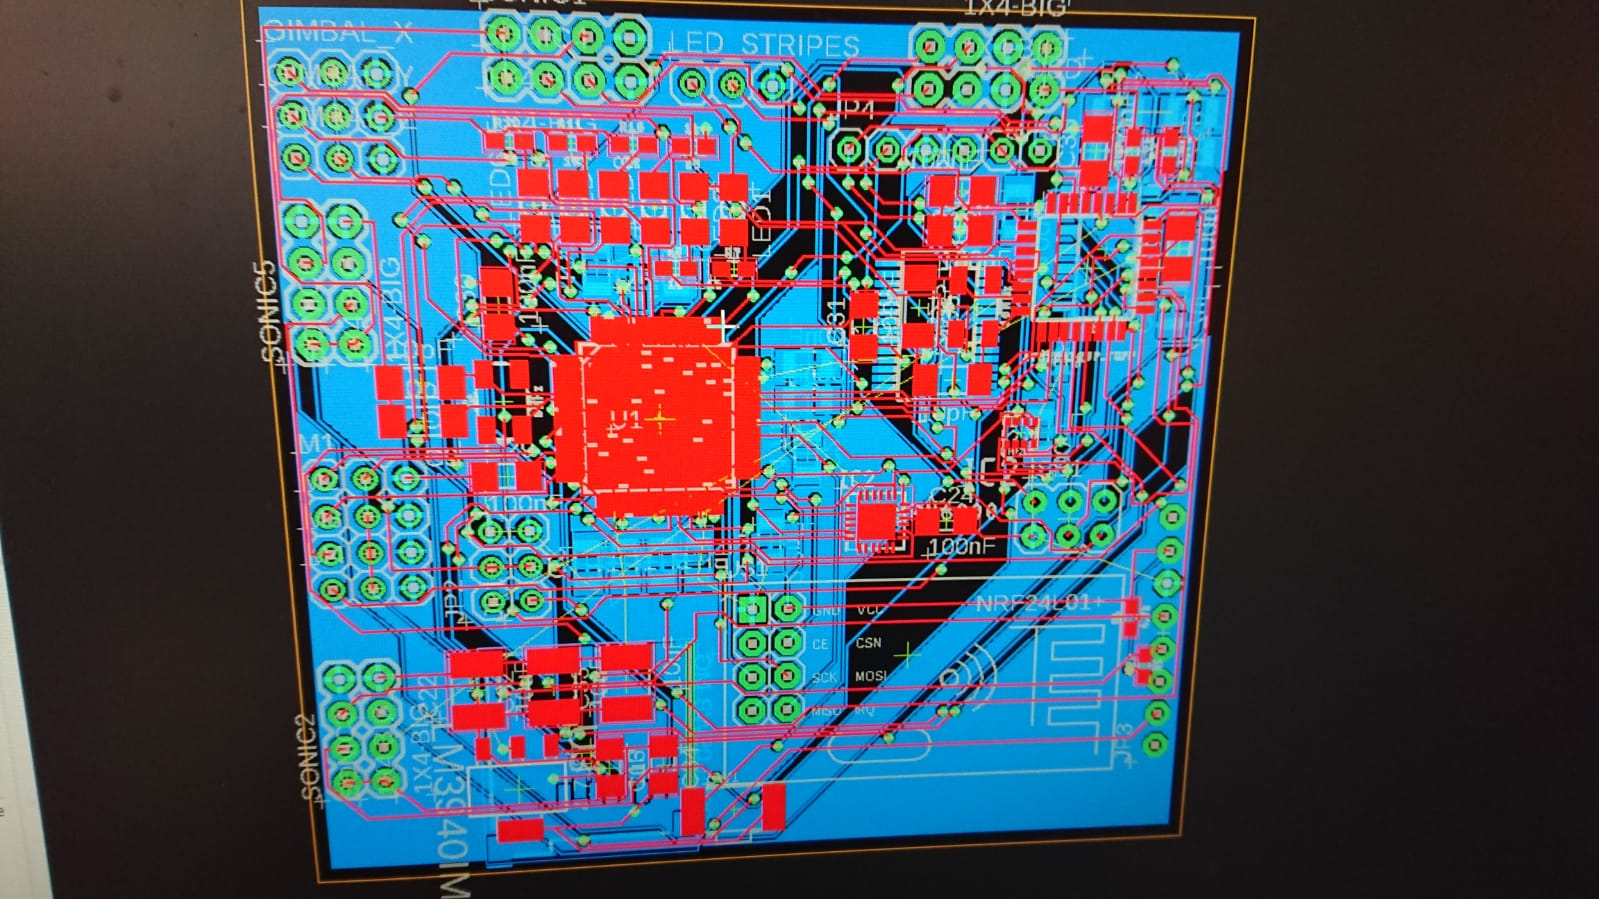
\includegraphics[width=1\textwidth]{Board(1).jpg}
\end{center}
\column{0.5\textwidth}
\begin{center}
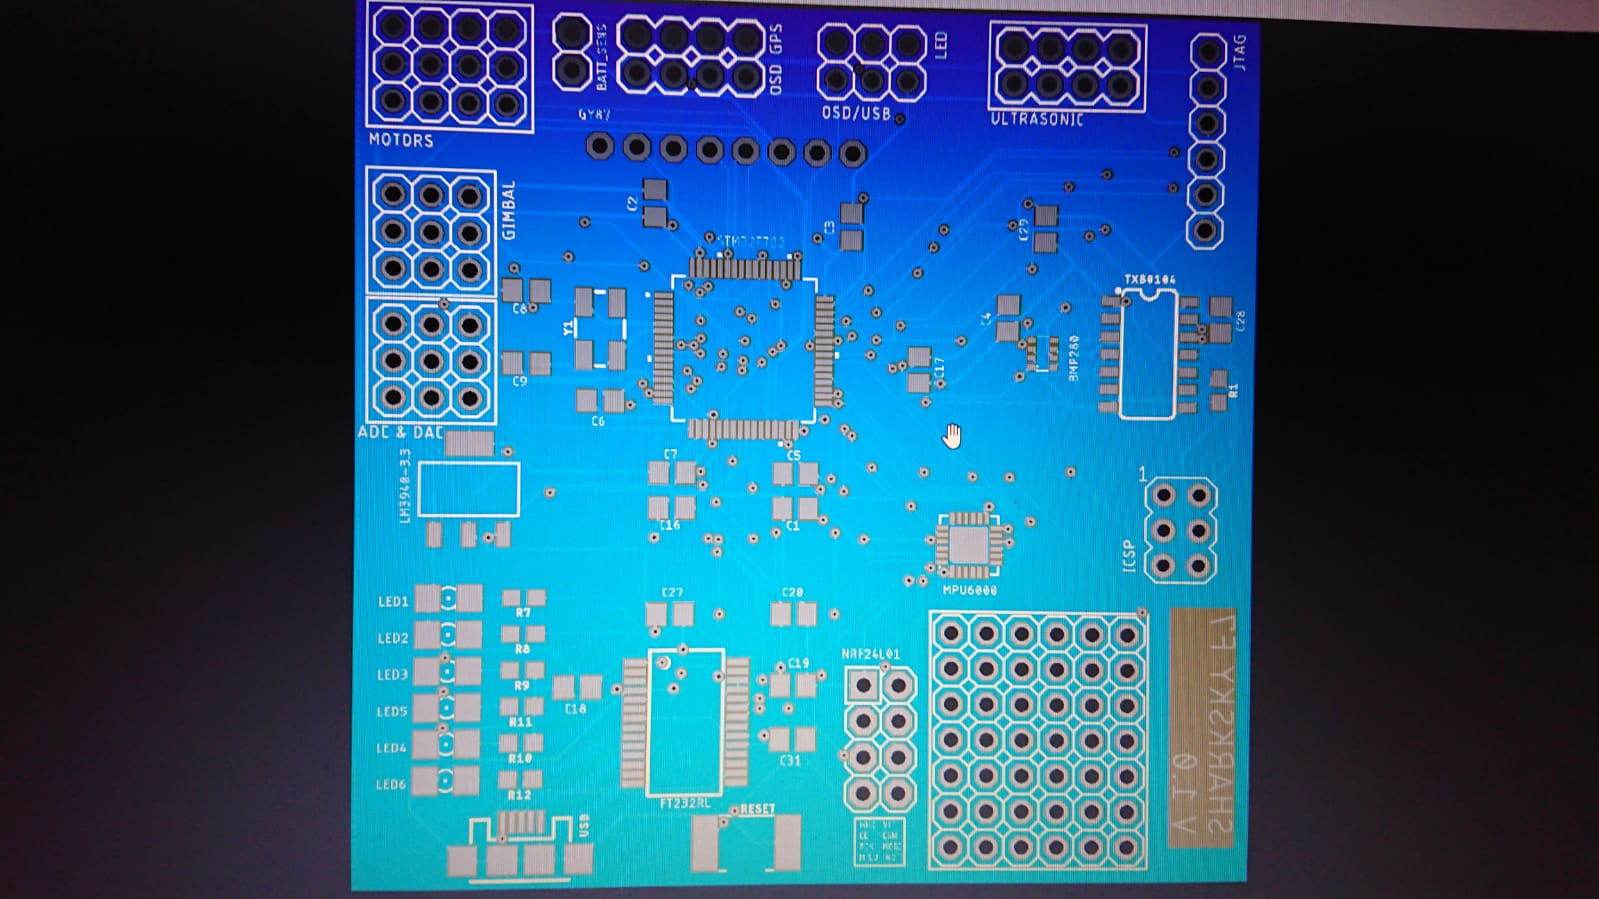
\includegraphics[width=1\textwidth]{Board(2).jpg}
\end{center}
\end{columns}
\end{frame}

\begin{frame}
\frametitle{Bau - Bilder}
Negativ
\end{frame}

\begin{frame}
Board
\end{frame}

\begin{frame}
\frametitle{Bau - Bilder}
\begin{columns}
\column{0.5\textwidth}
\begin{center}
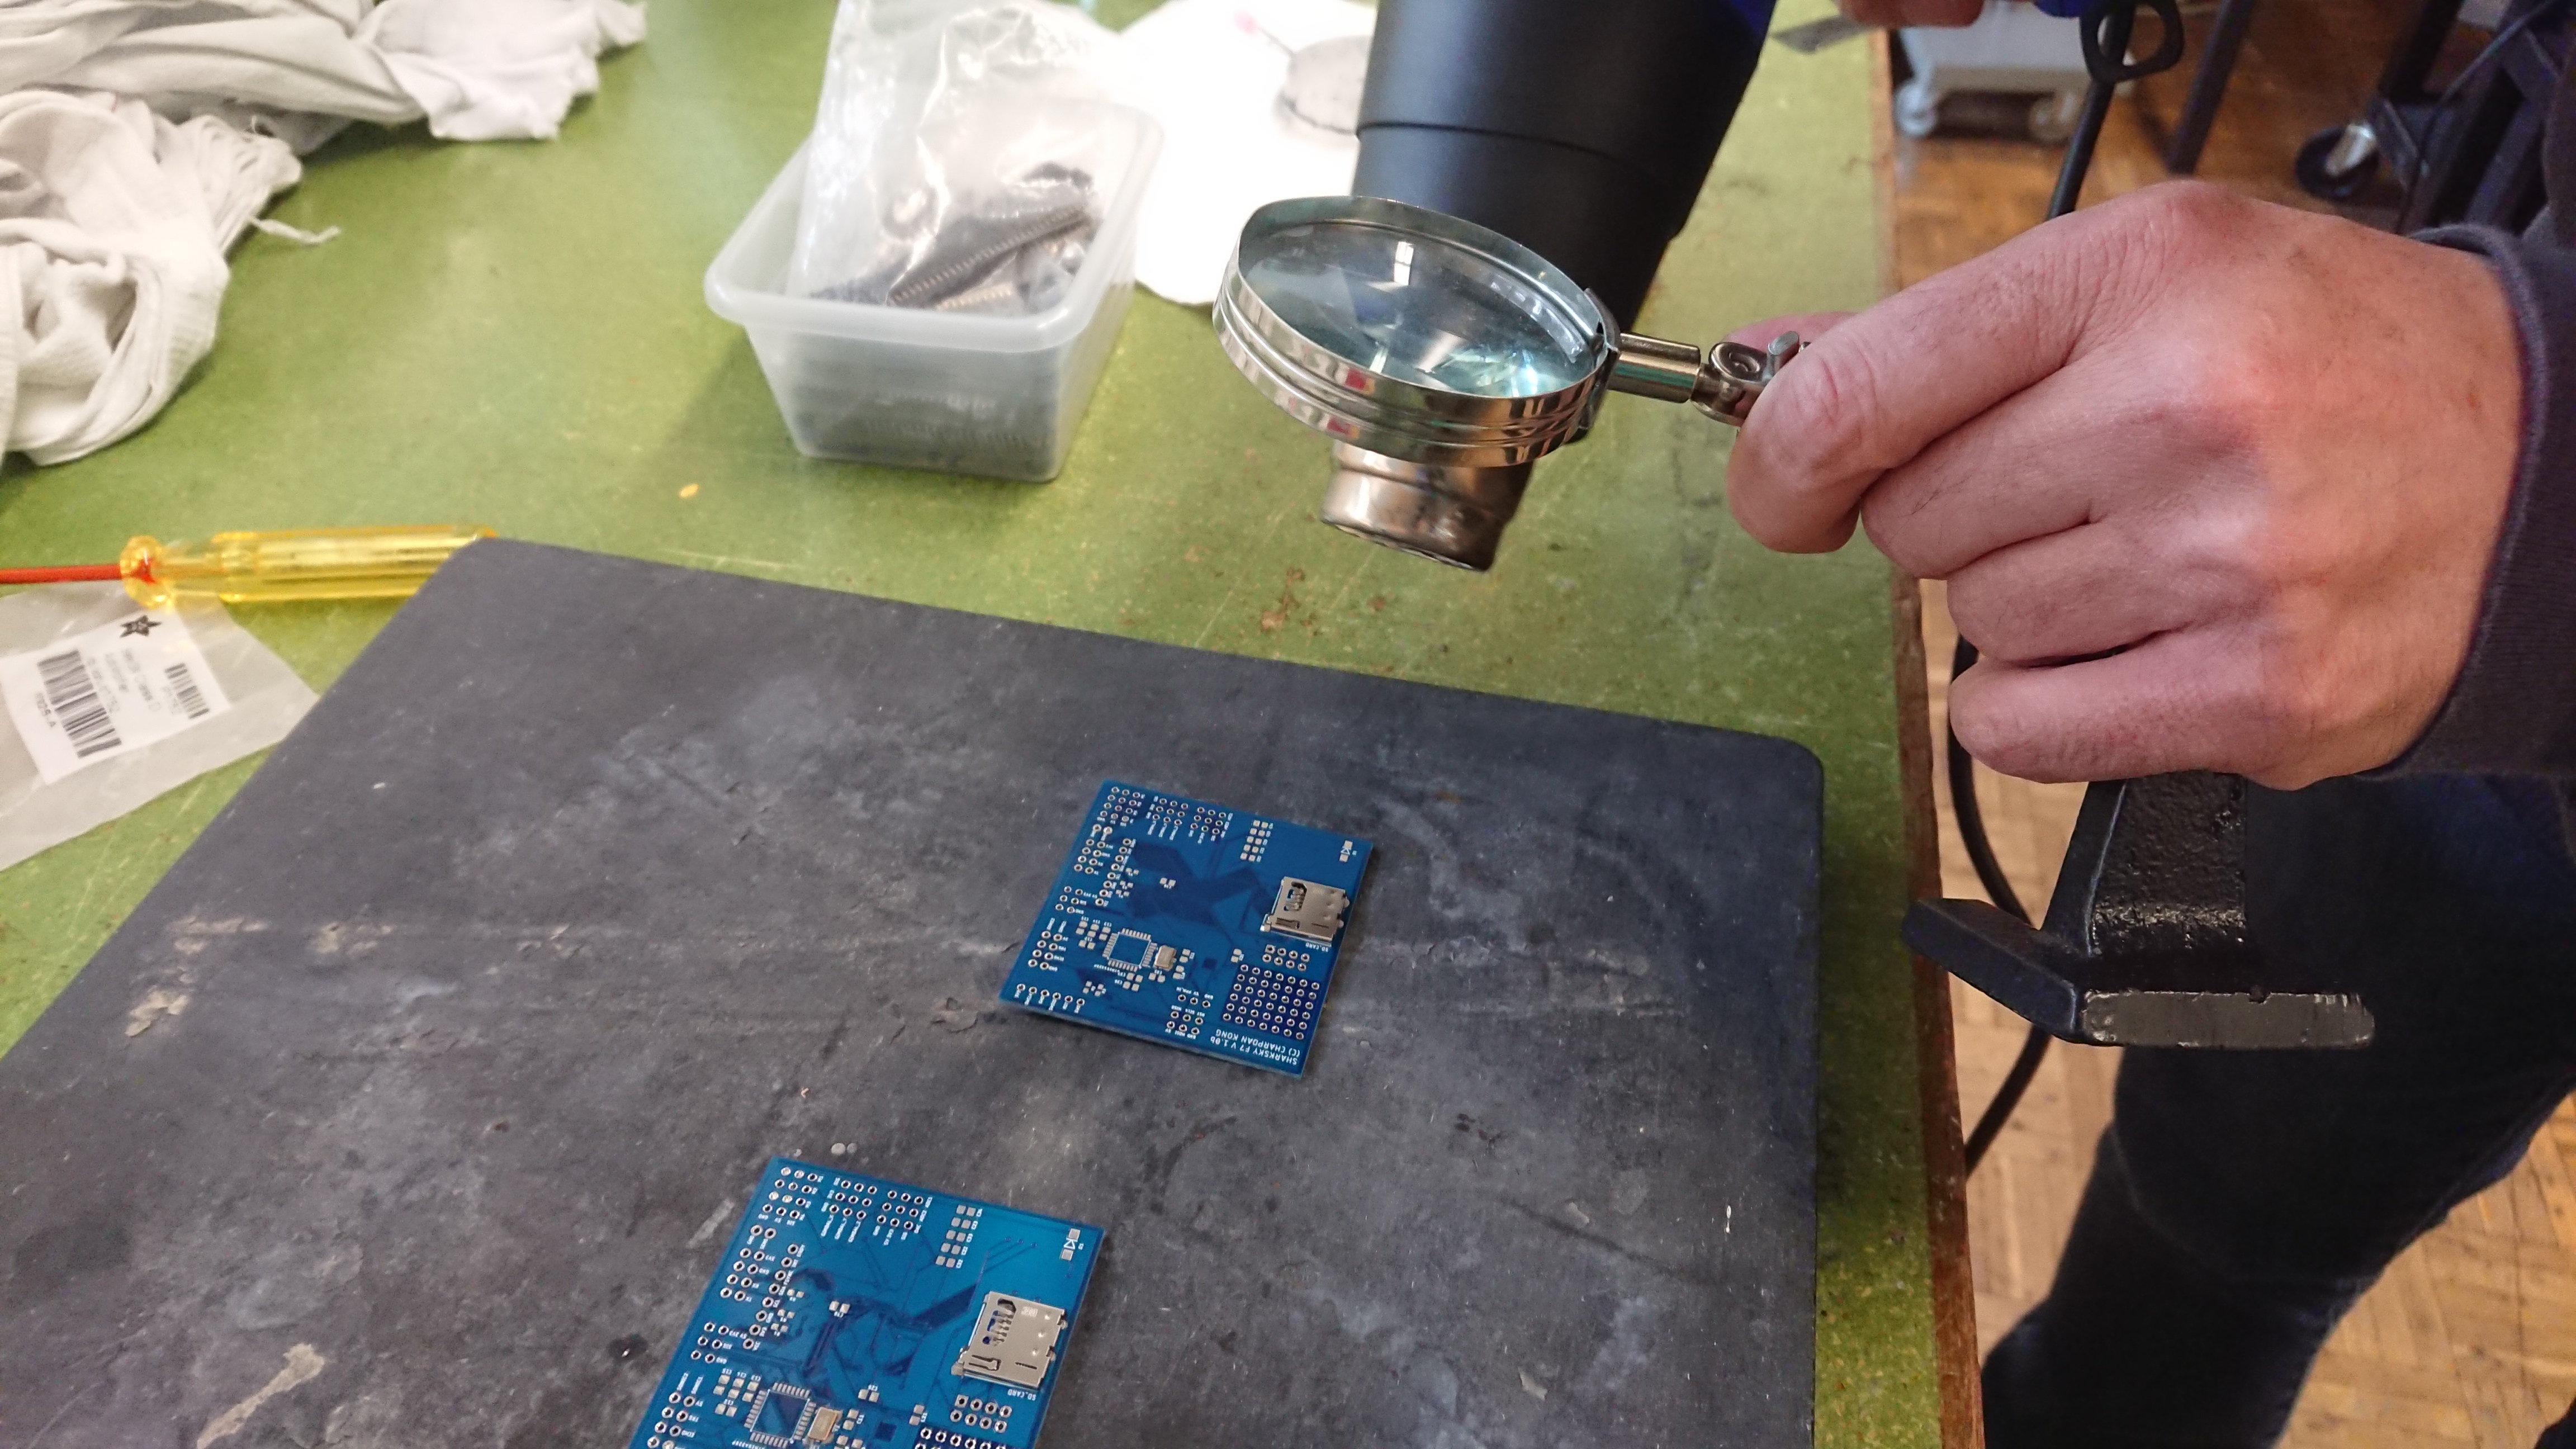
\includegraphics[width=1\textwidth]{LOET (1).JPG}
\end{center}
\column{0.5\textwidth}
\begin{center}
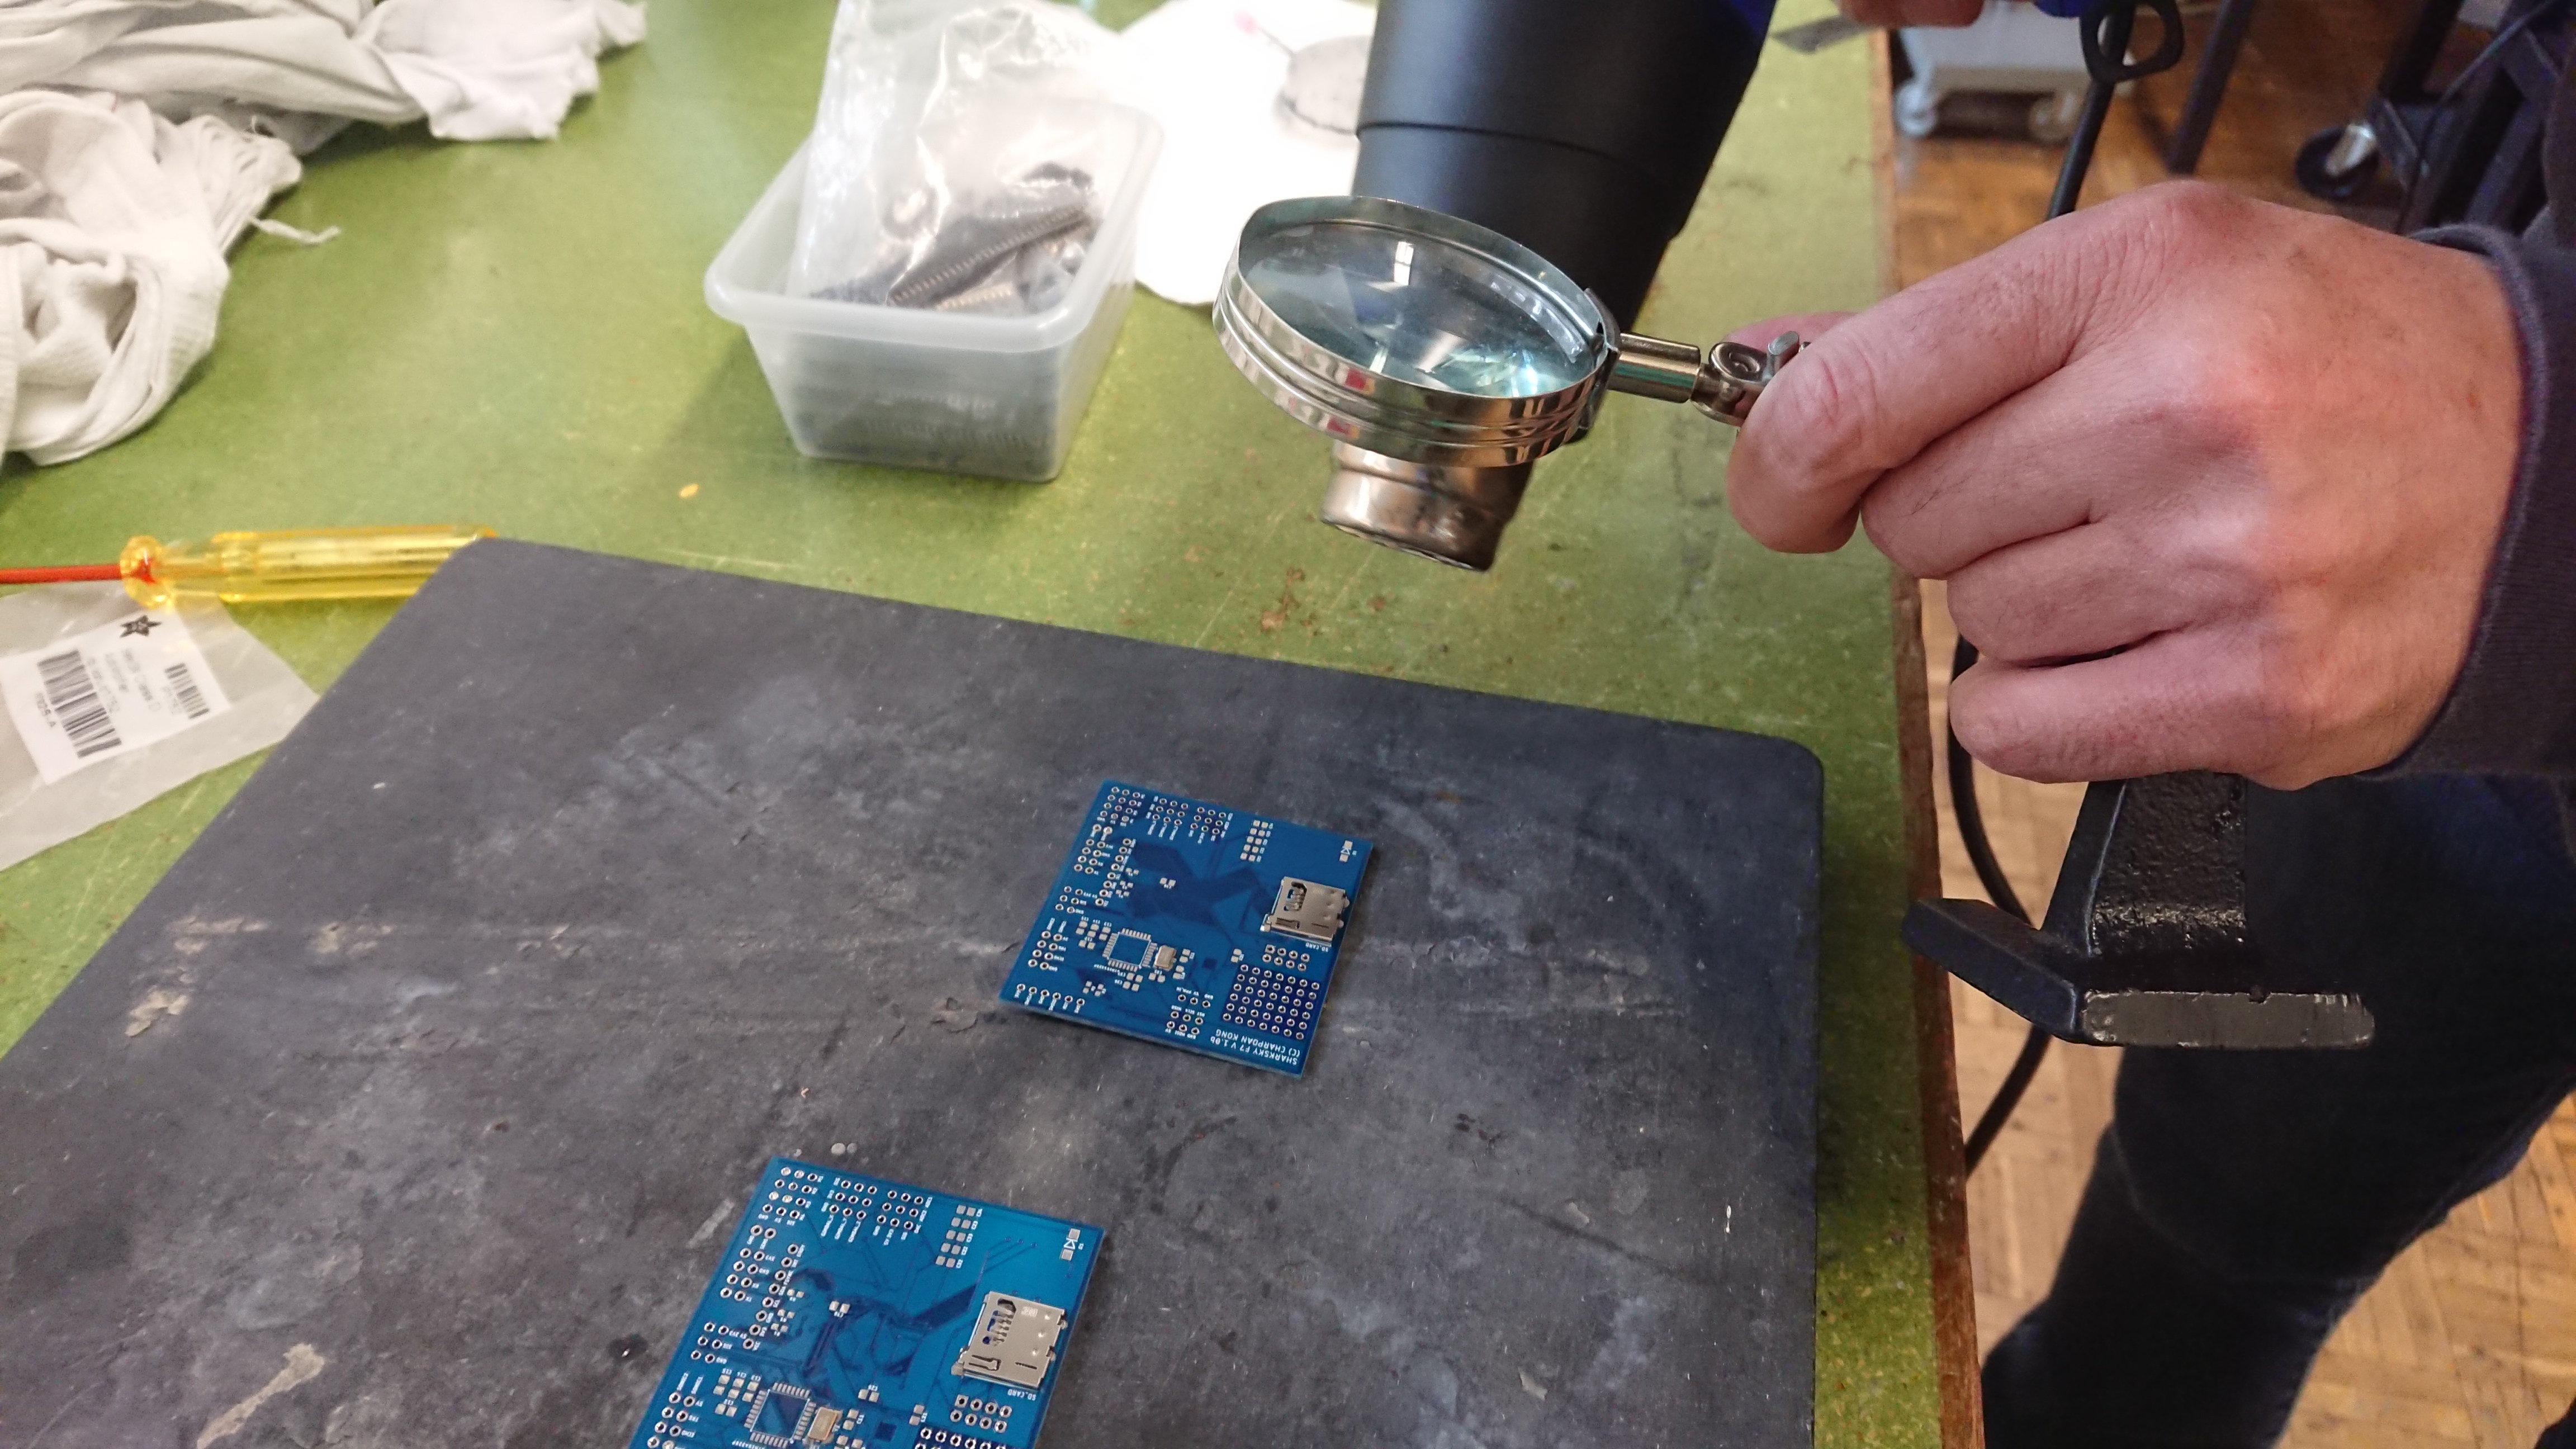
\includegraphics[width=1\textwidth]{LOET (2).JPG}
\end{center}
\end{columns}
\end{frame}

\begin{frame}
\frametitle{Bau - Bilder}
\begin{columns}
\column{0.5\textwidth}
\begin{center}
\includegraphics[width=1\textwidth]{LOET (3).JPG}
\end{center}
\column{0.5\textwidth}
\begin{center}
\includegraphics[width=1\textwidth]{LOET (4).JPG}
\end{center}
\end{columns}
\end{frame}

\begin{frame}
\frametitle{Bau - Bilder}
\begin{columns}
\column{0.5\textwidth}
\begin{center}
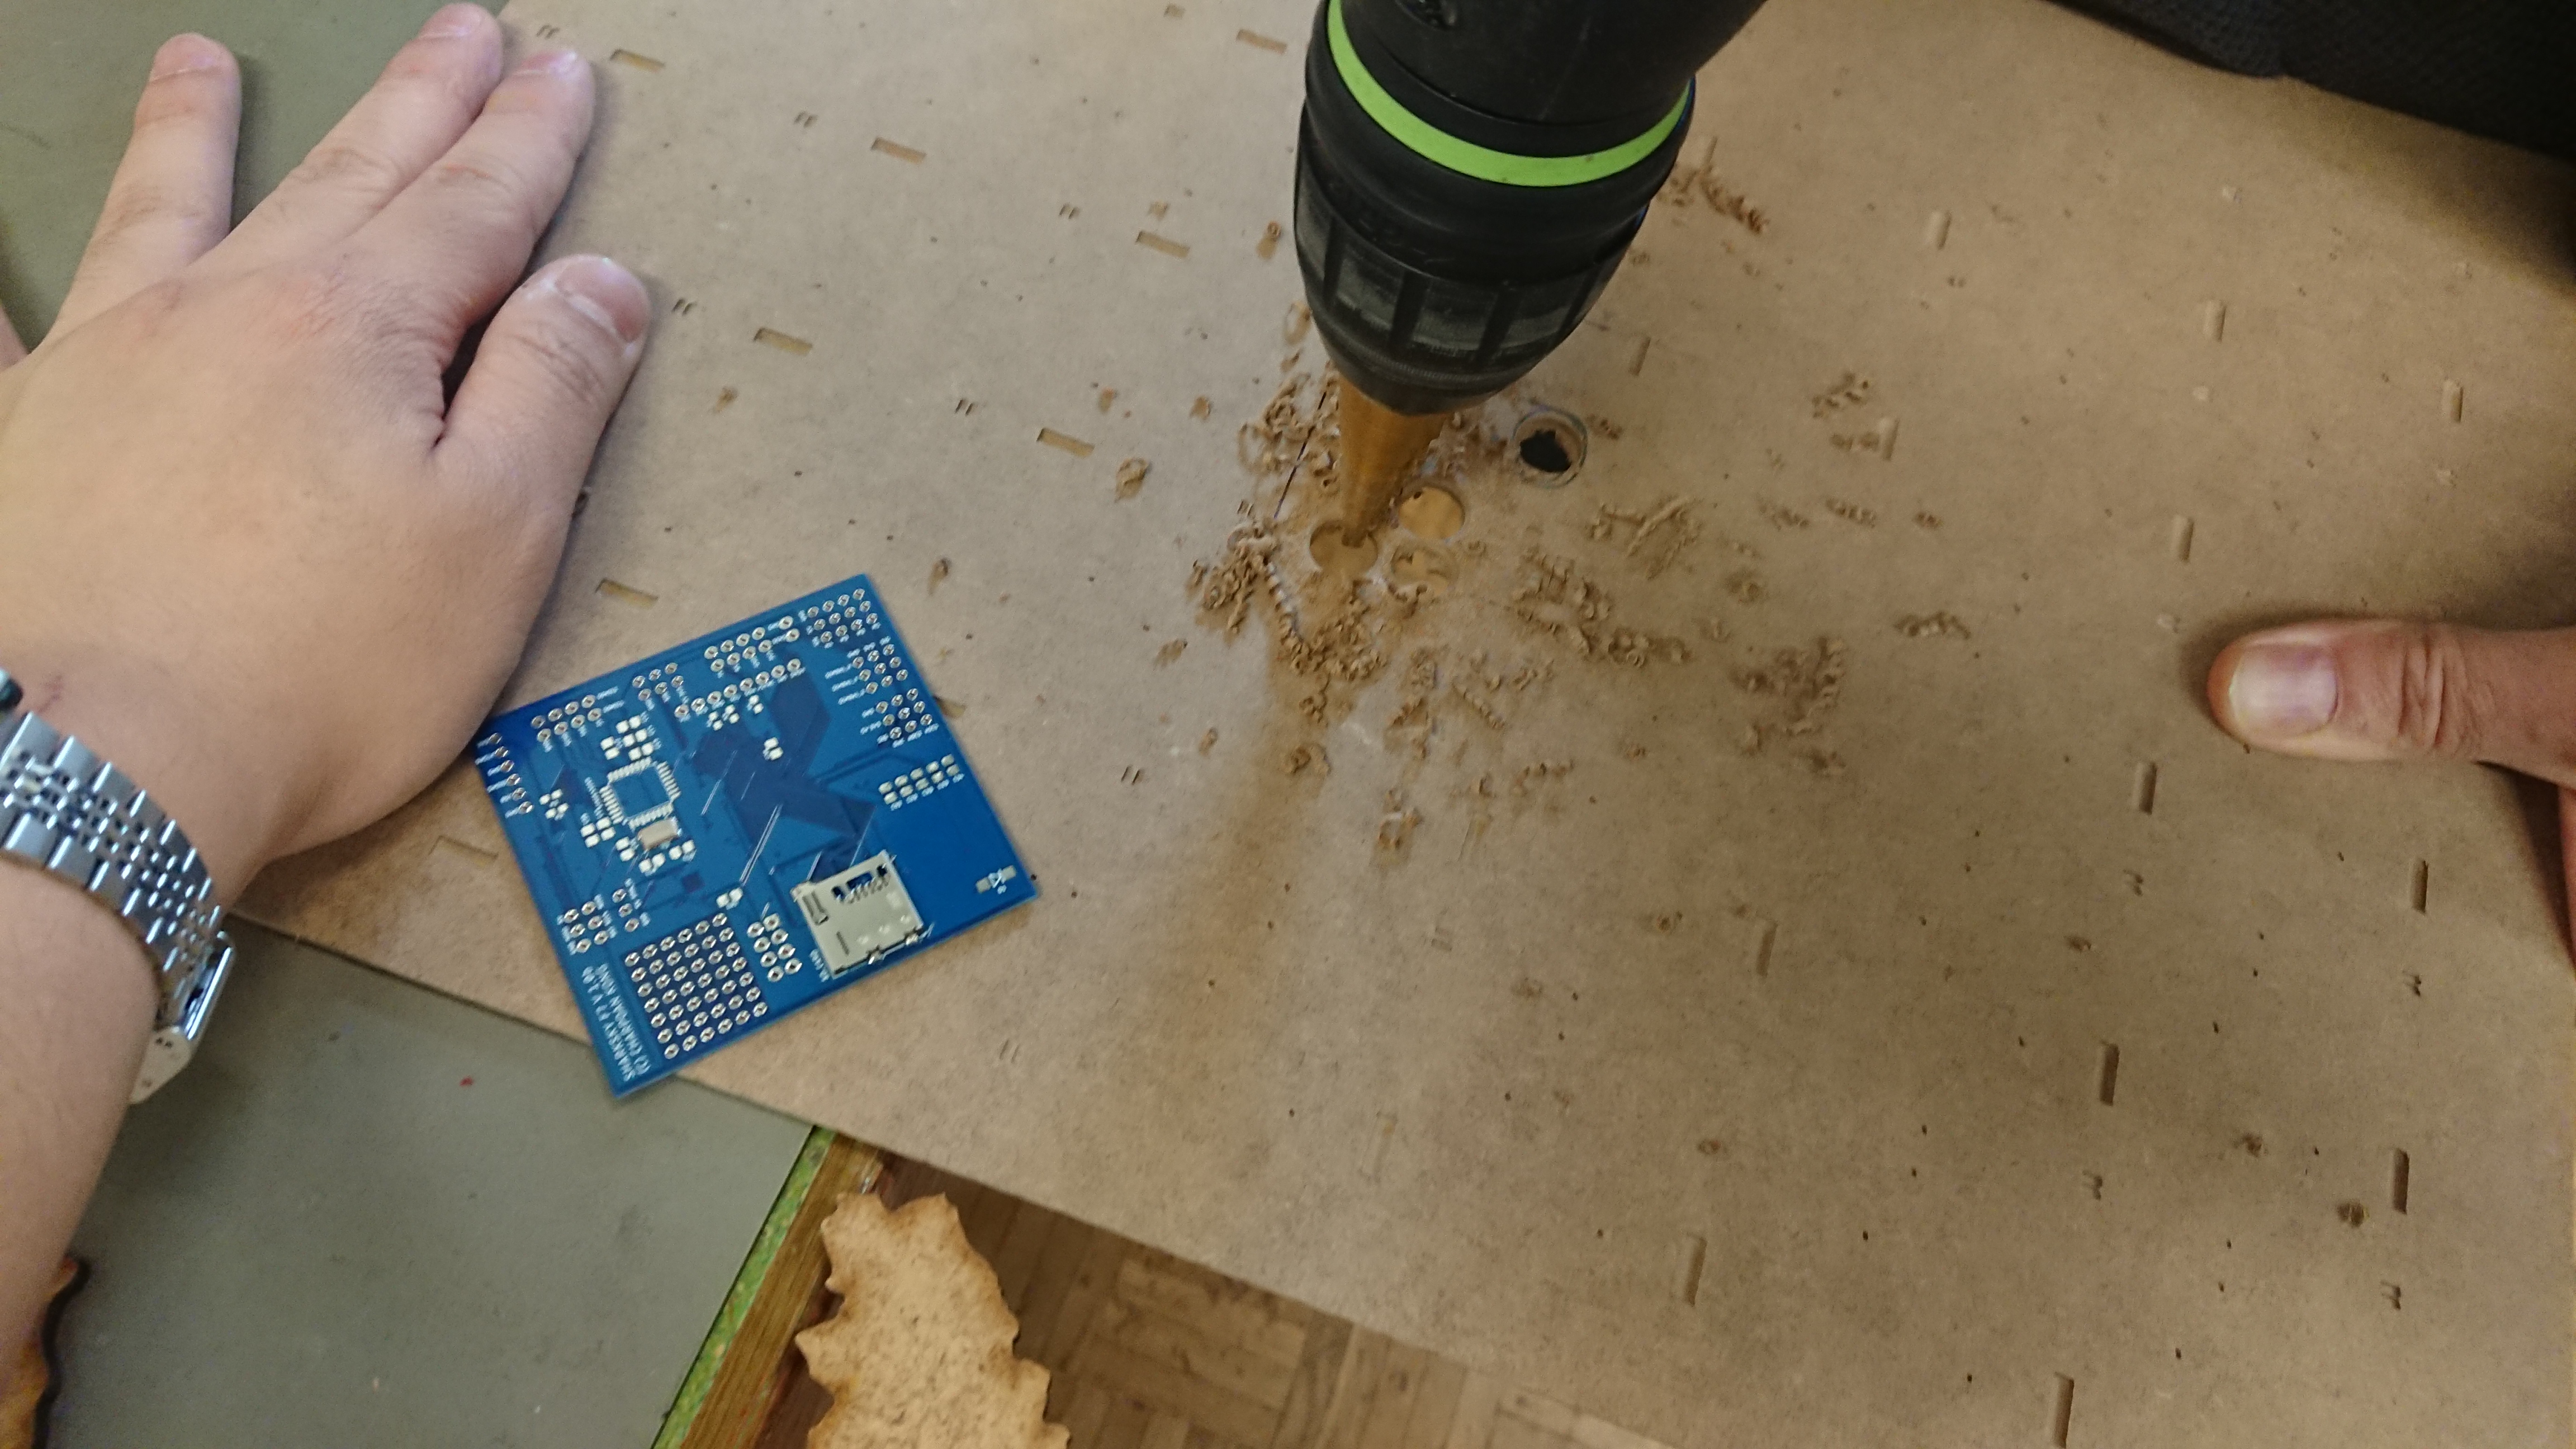
\includegraphics[width=1\textwidth]{LOET (6).JPG}
\end{center}
\column{0.5\textwidth}
\begin{center}
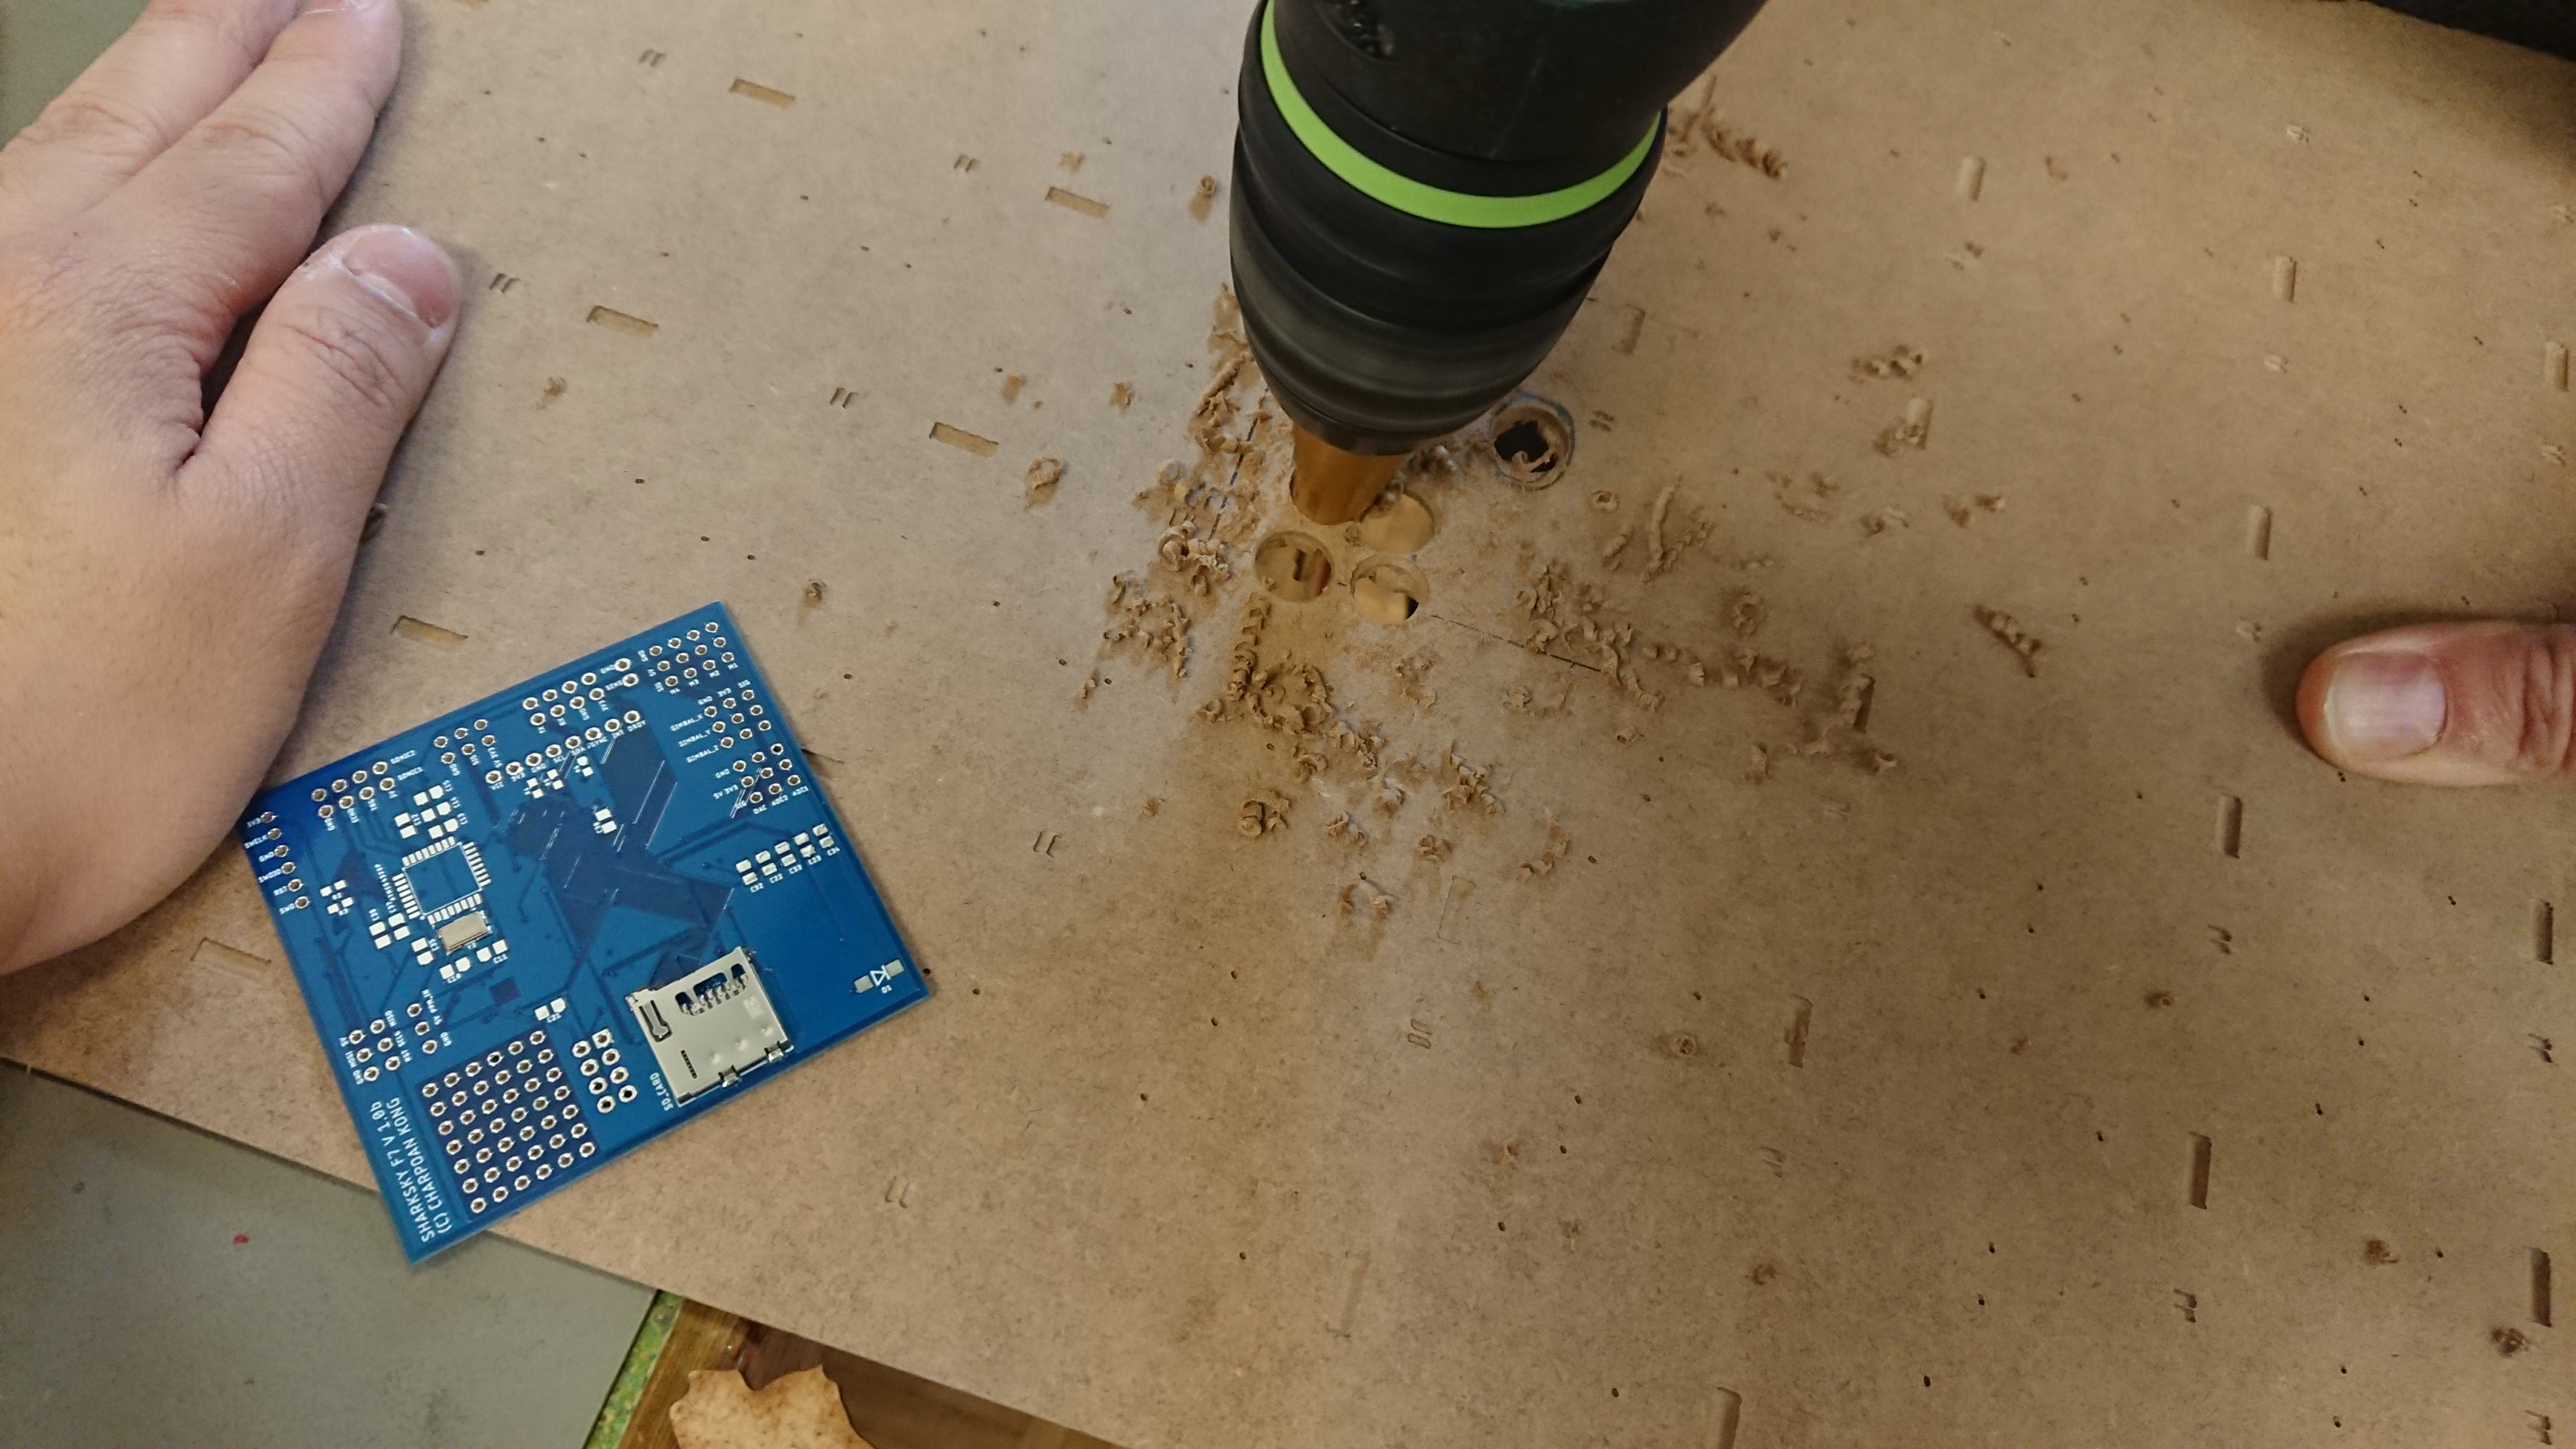
\includegraphics[width=1\textwidth]{LOET (7).JPG}
\end{center}
\end{columns}
\end{frame}

\begin{frame}
\frametitle{Bau - Bilder}
\begin{center}
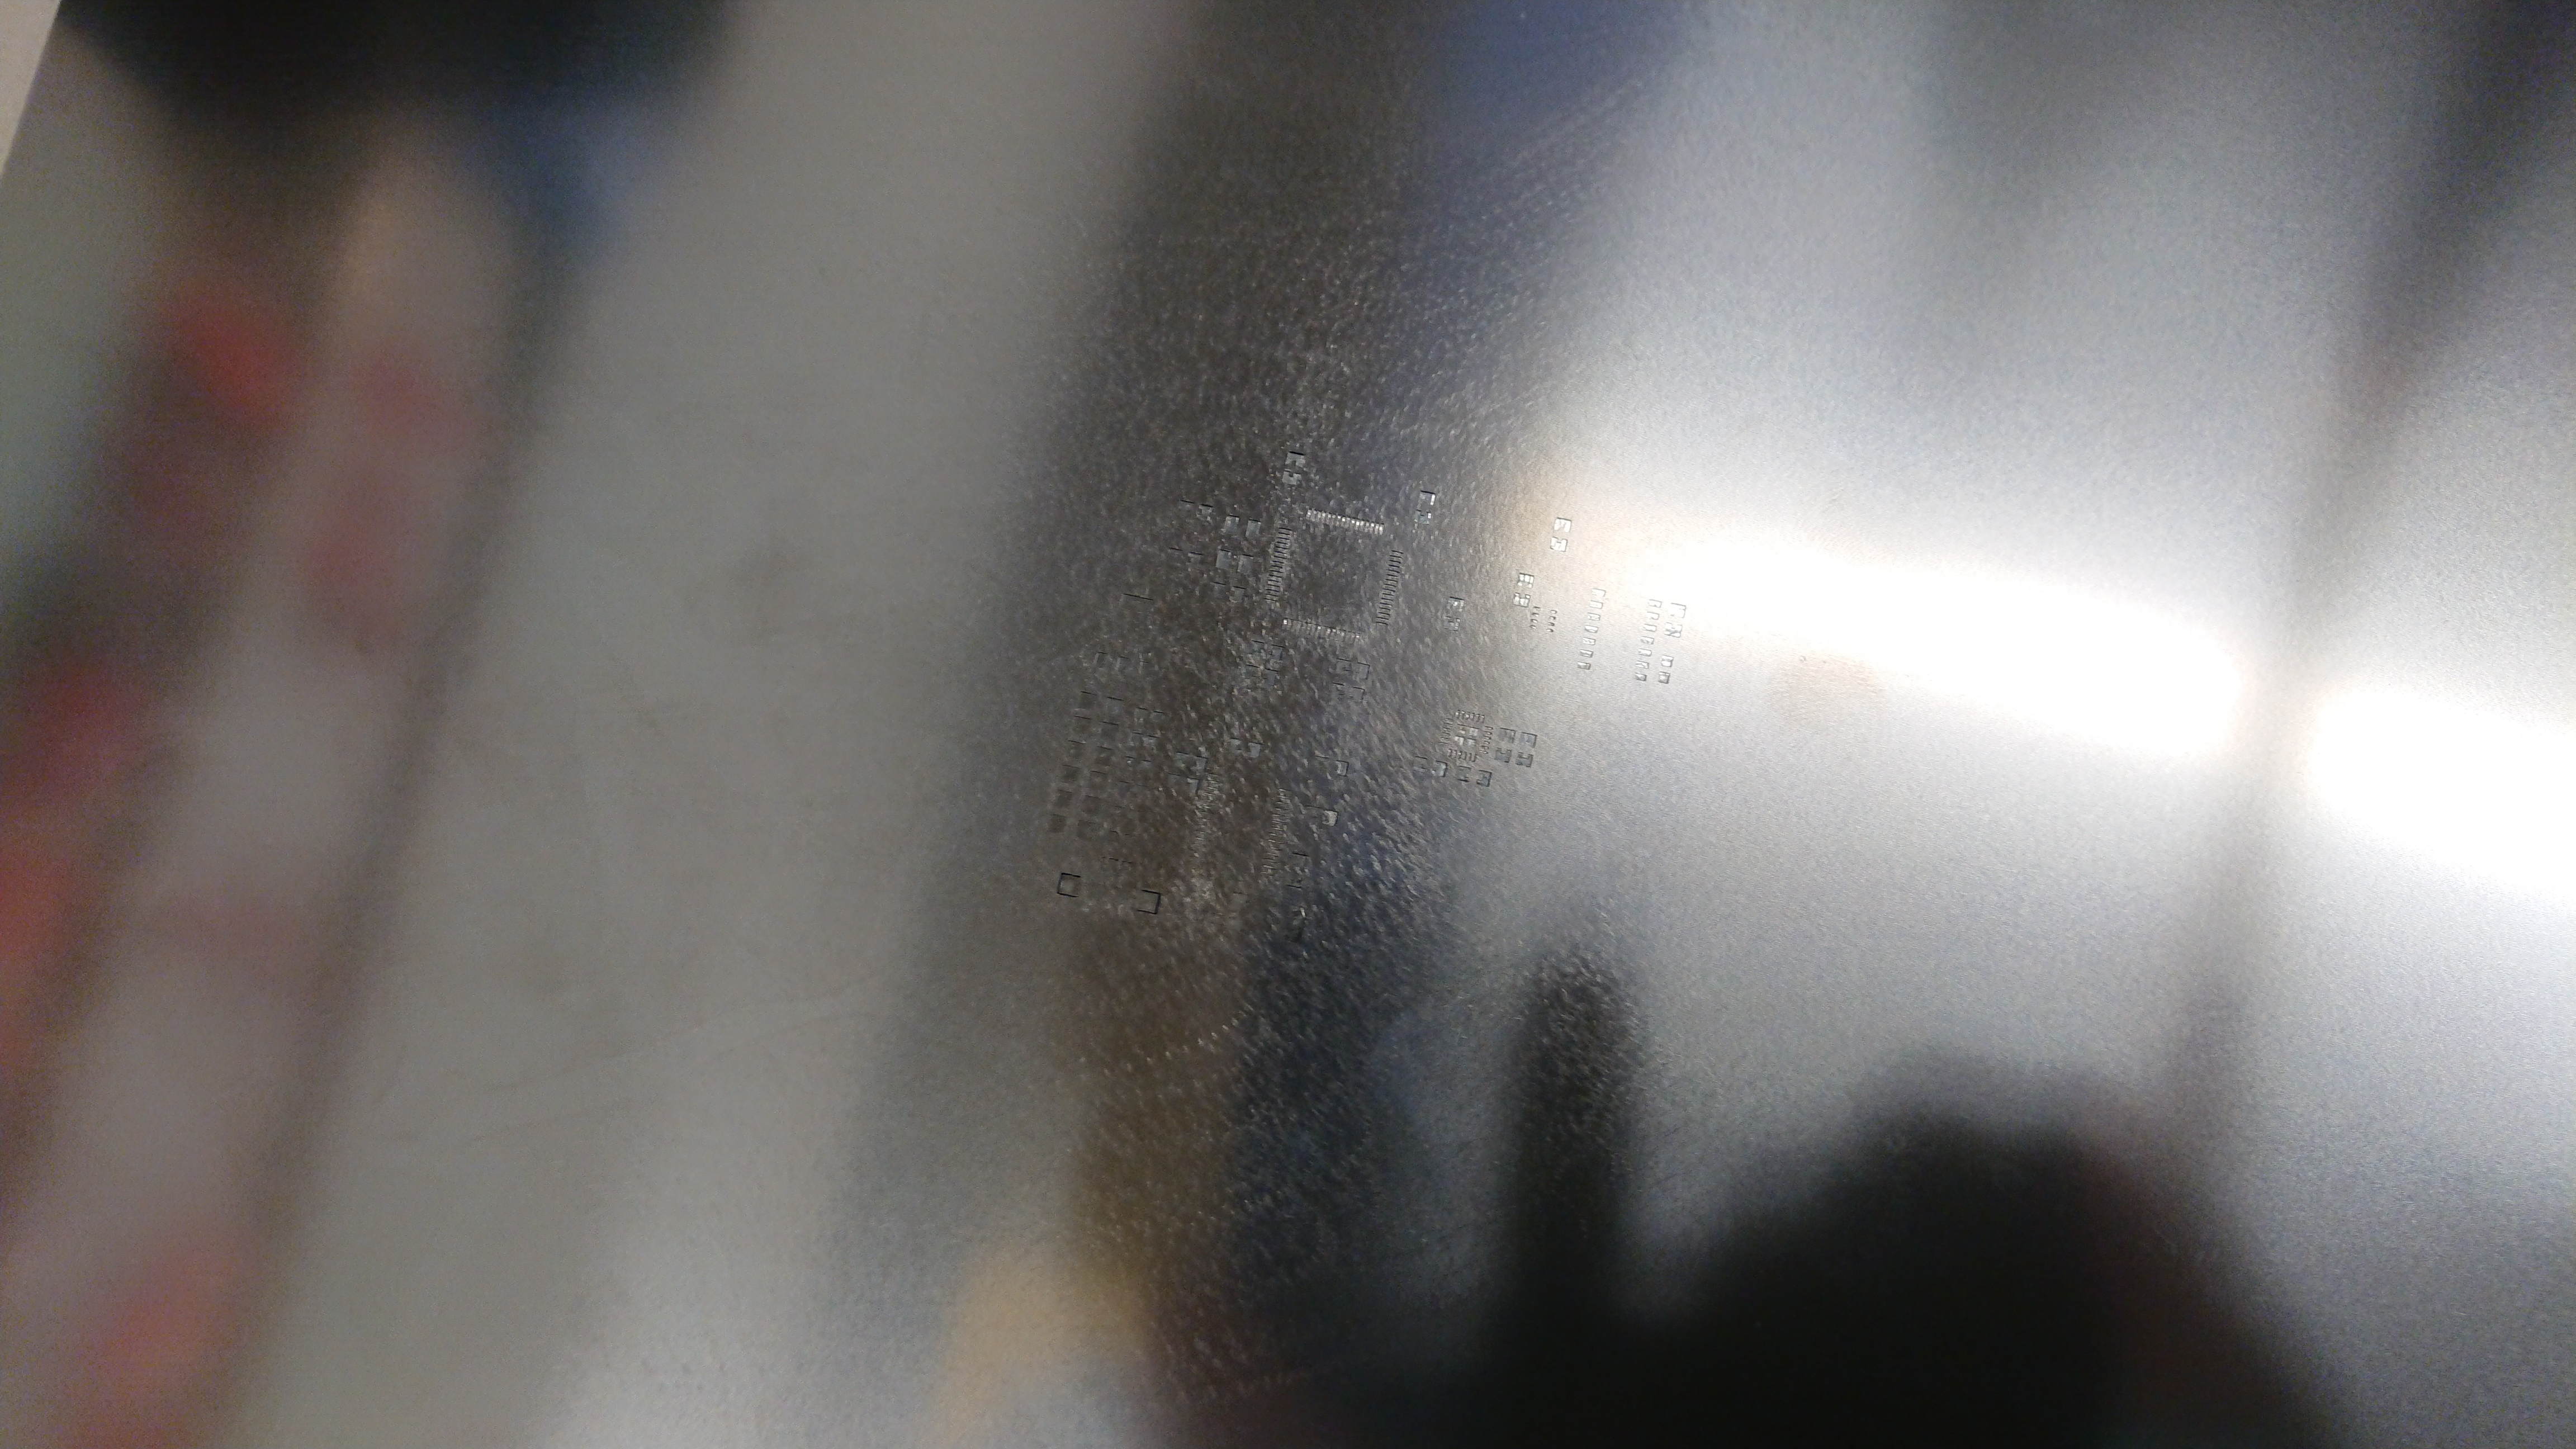
\includegraphics[width=1\textwidth]{LOET (8).JPG}
\end{center}
\end{frame}

\begin{frame}
\frametitle{Bau - Bilder}
\begin{columns}
\column{0.5\textwidth}
\begin{center}
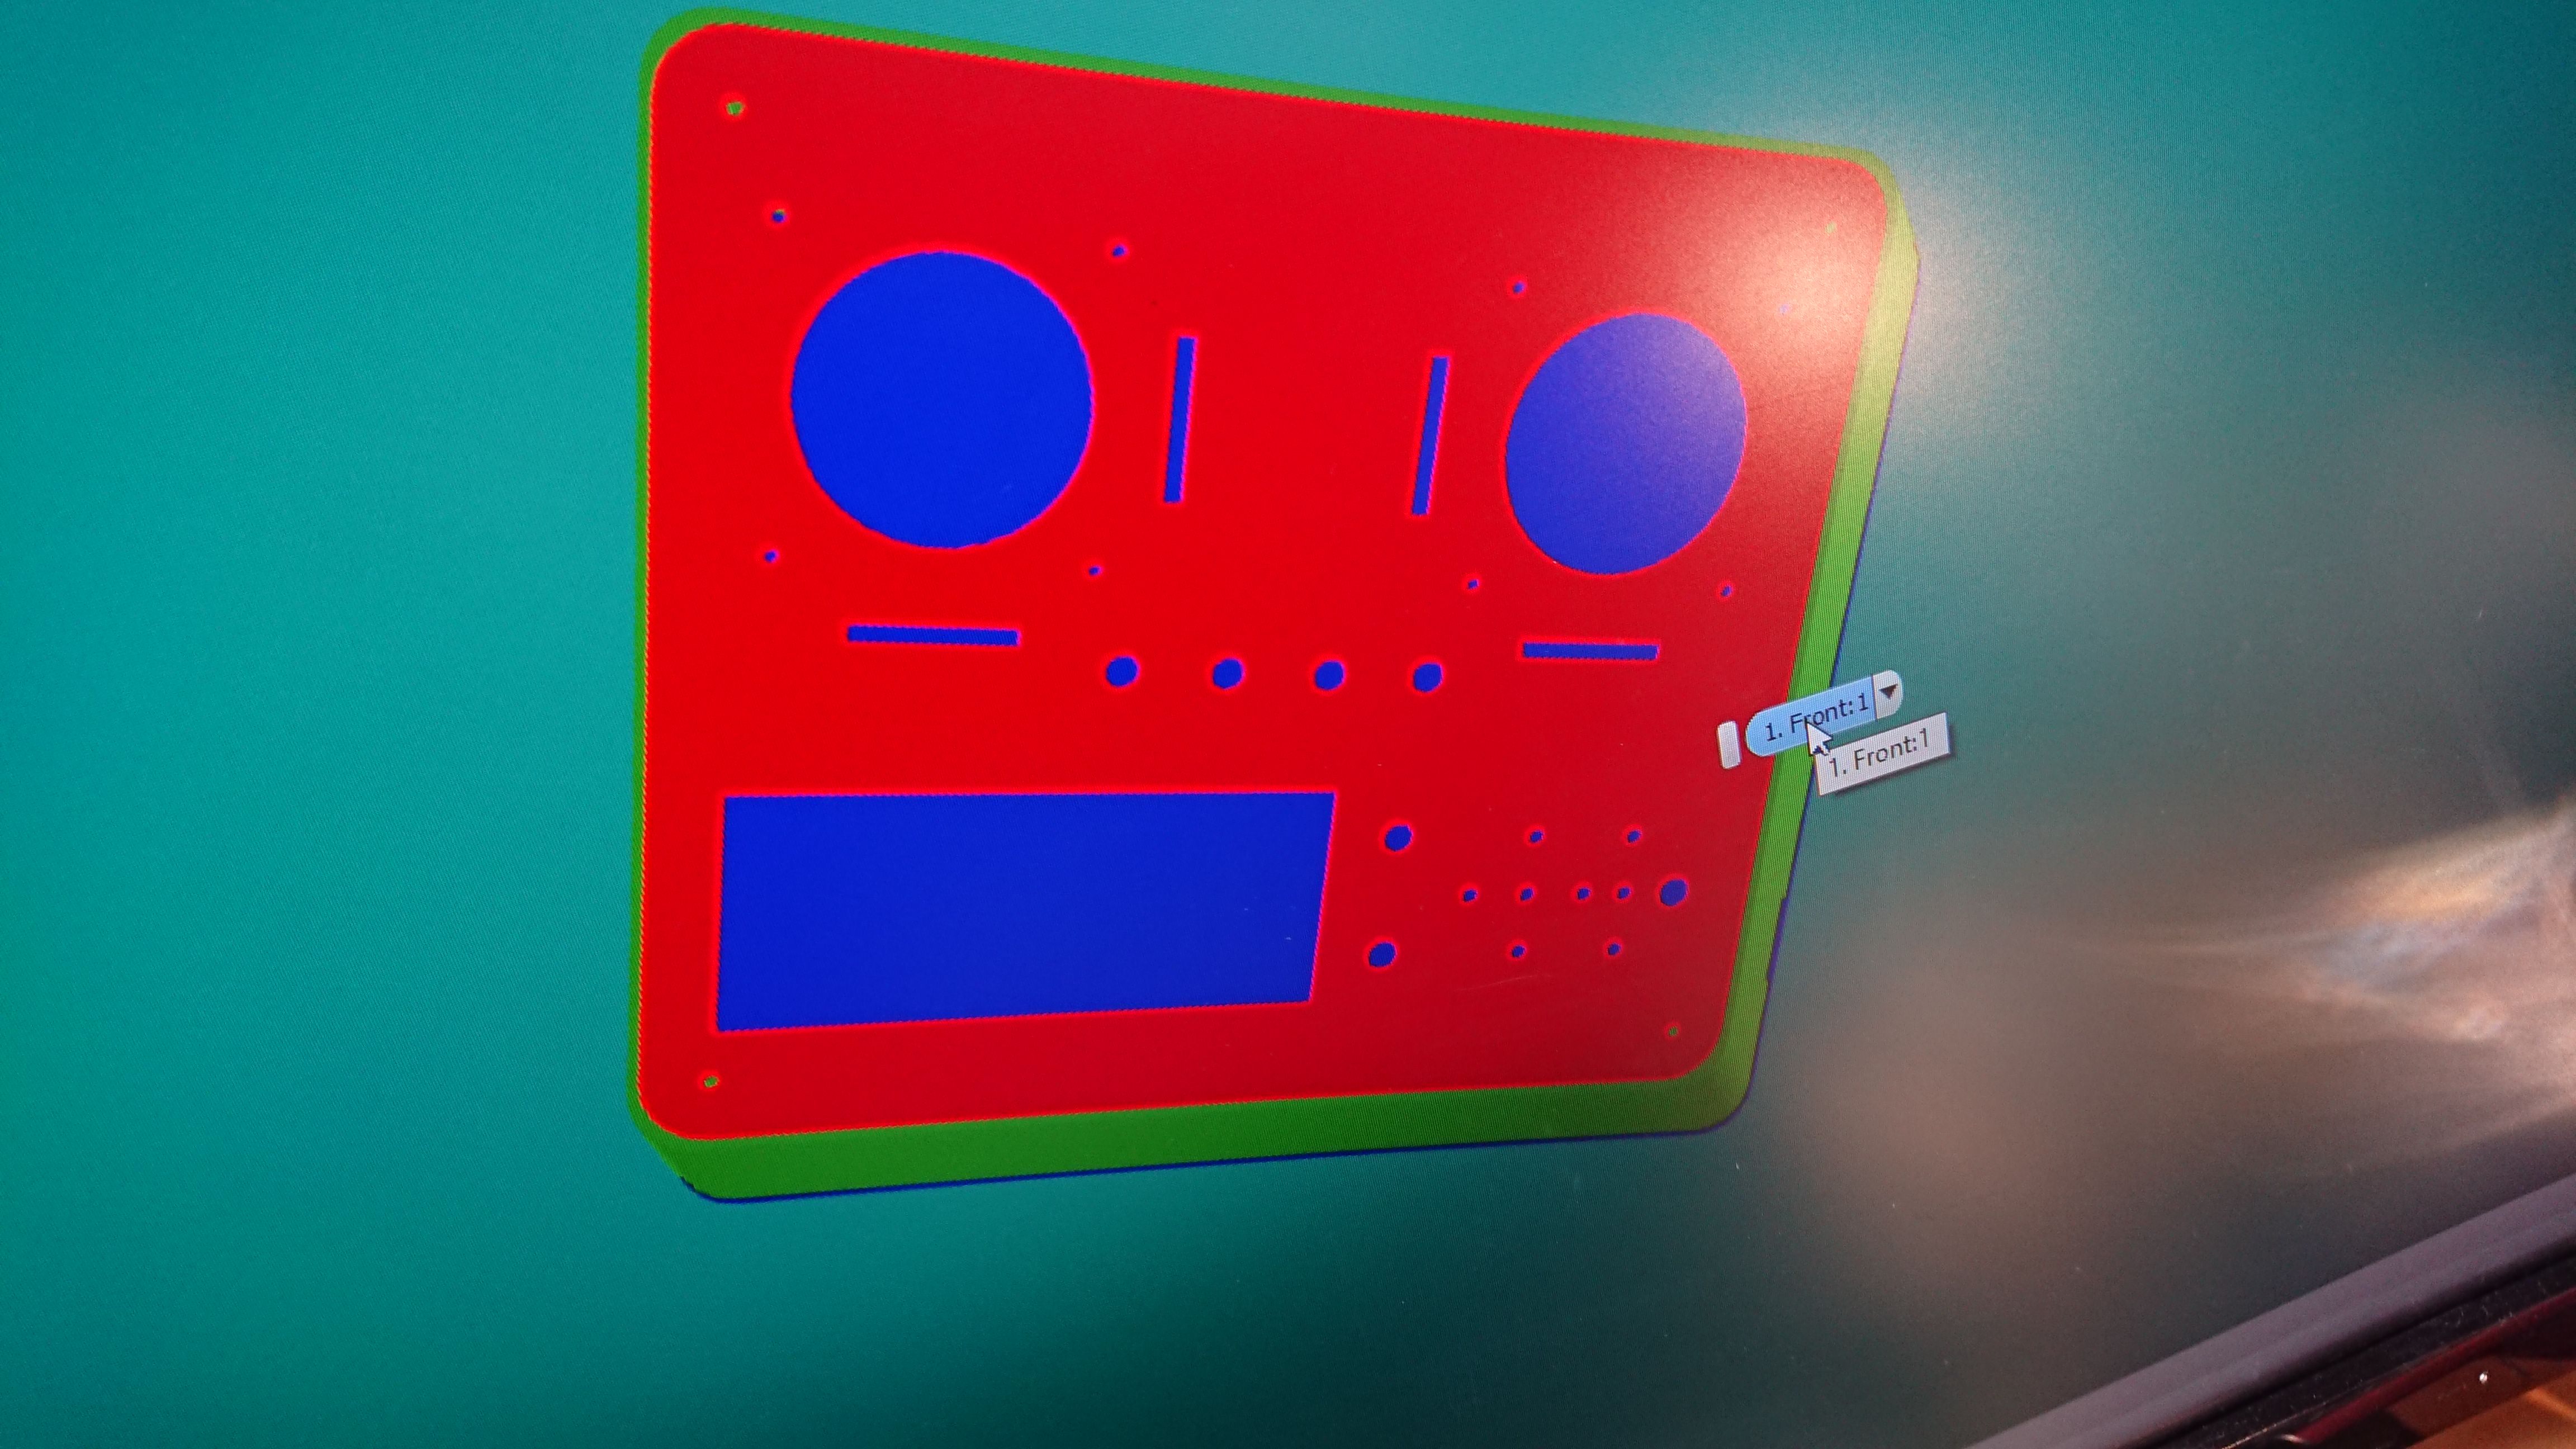
\includegraphics[width=1\textwidth]{Ferni (1).jpeg}
\end{center}
\column{0.5\textwidth}
\begin{center}
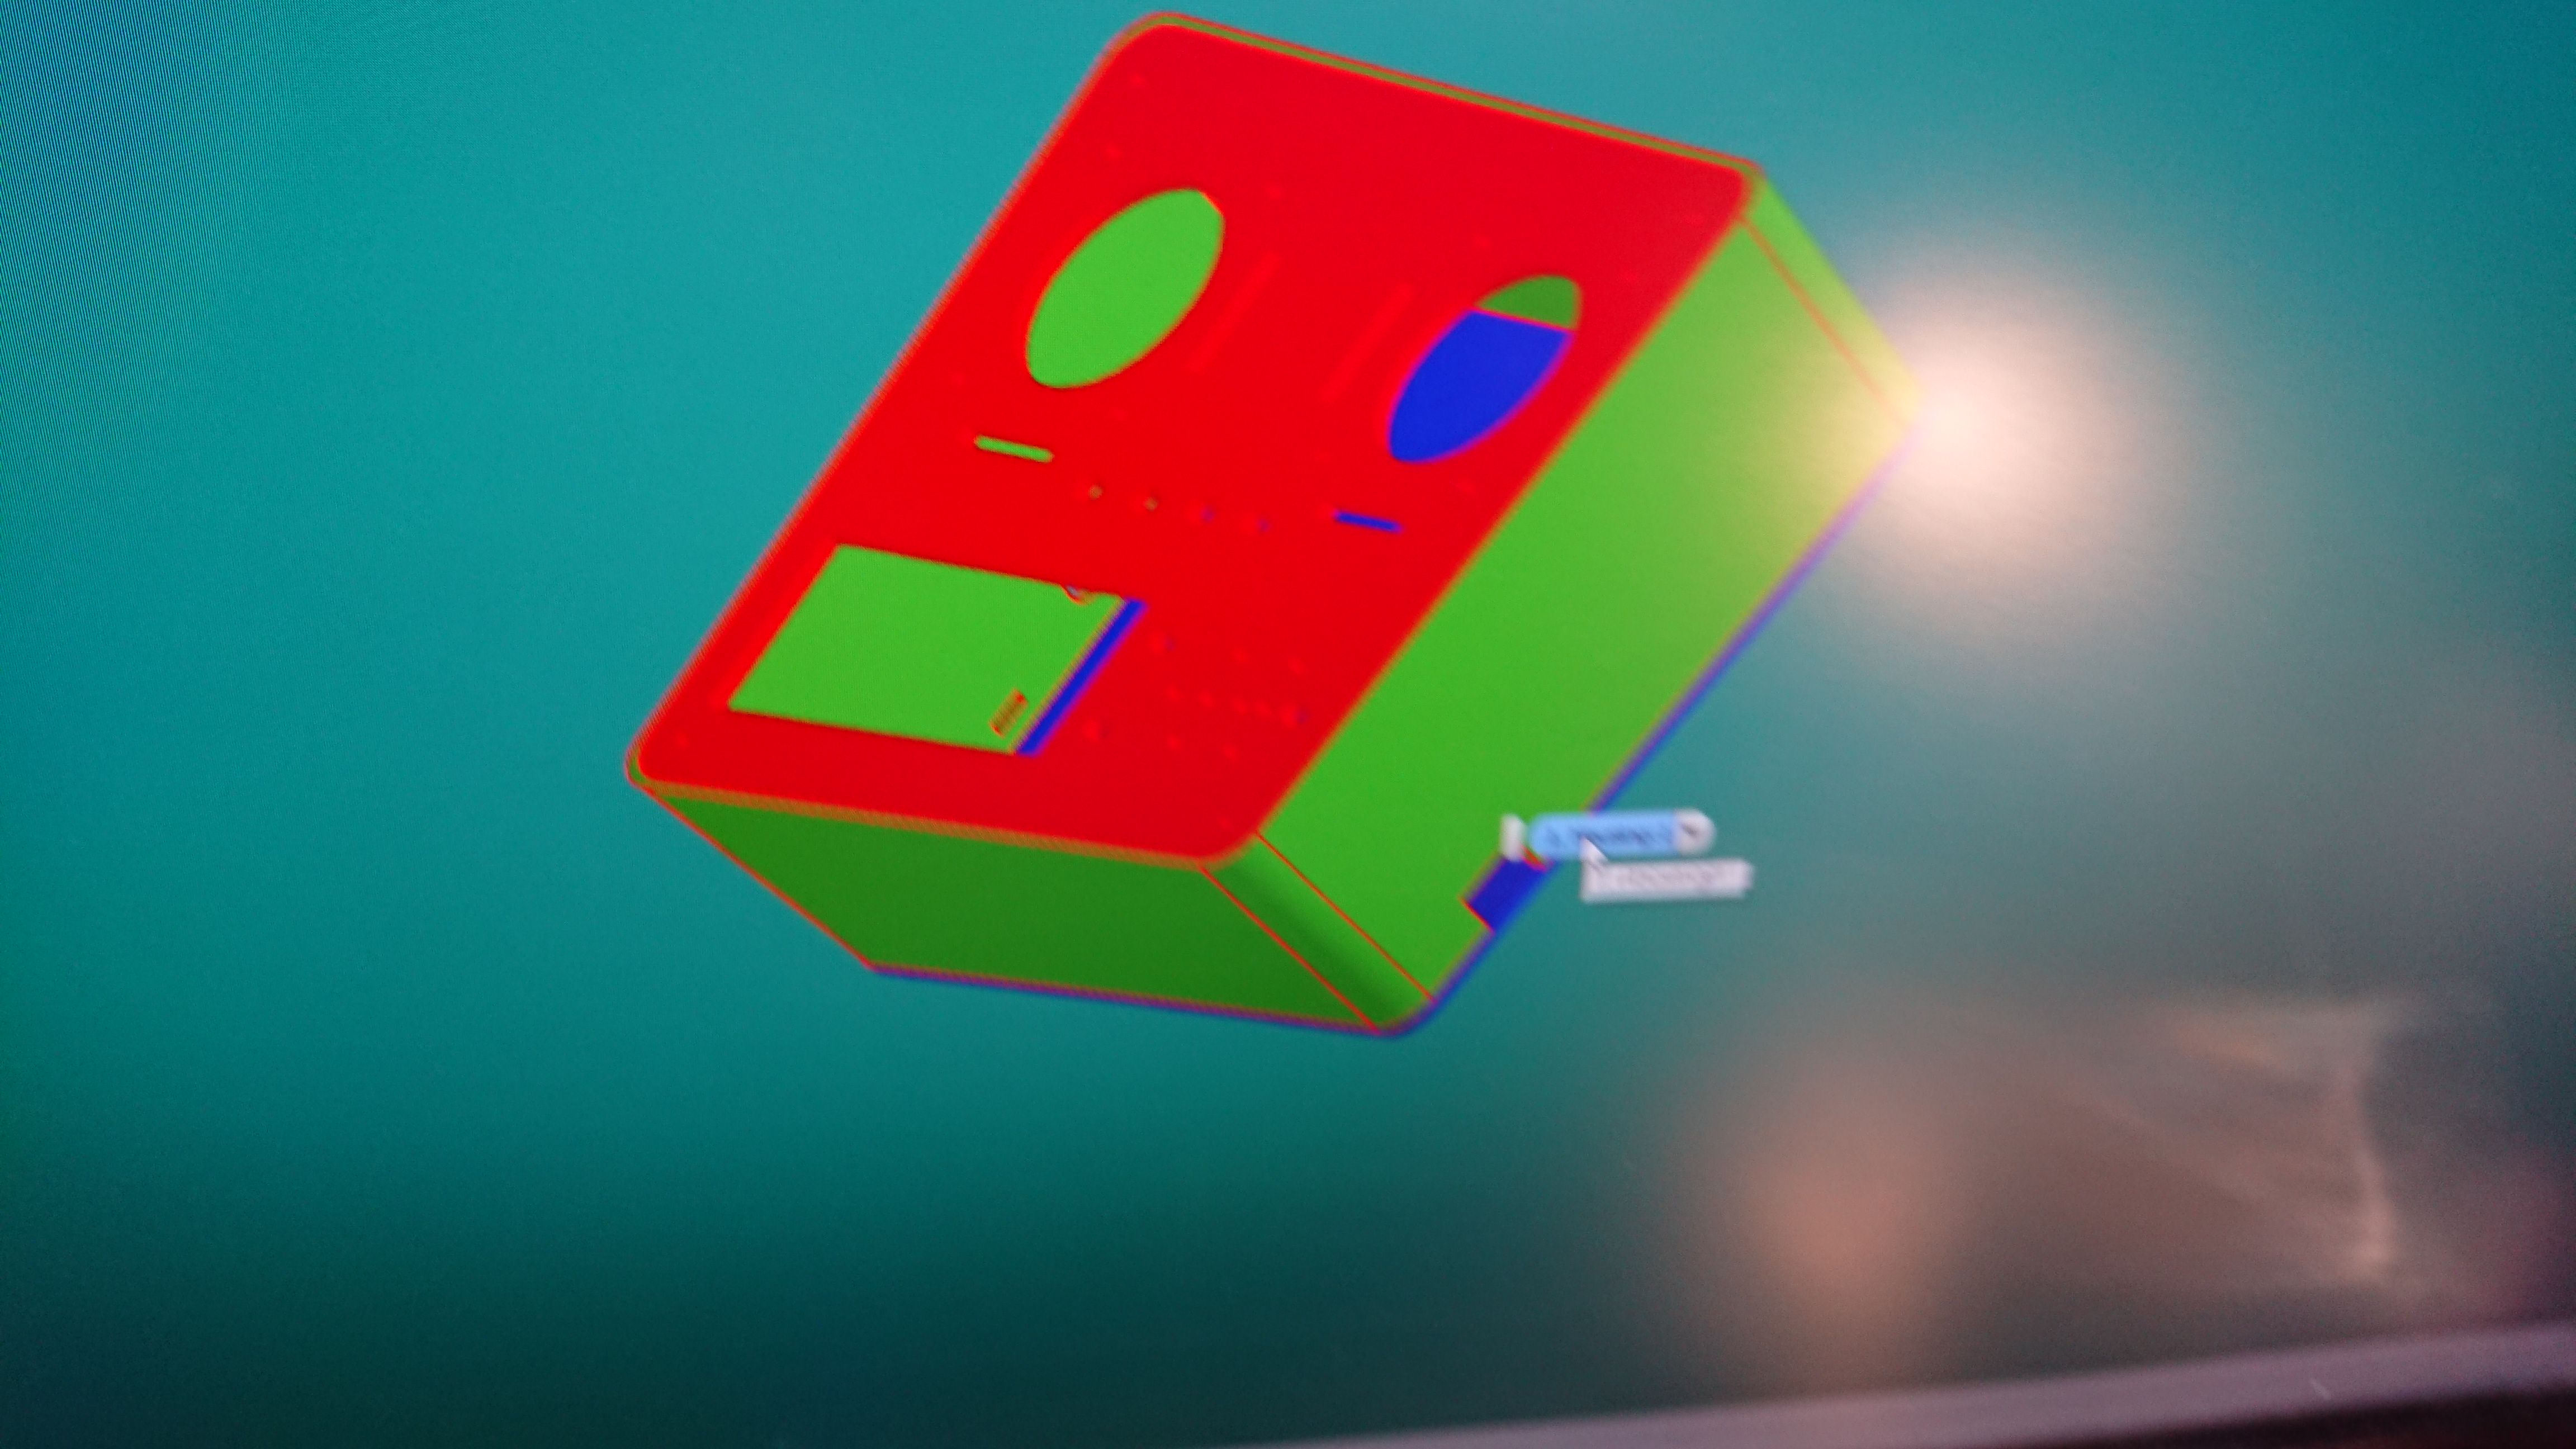
\includegraphics[width=1\textwidth]{Ferni (2).jpeg}
\end{center}
\end{columns}
\end{frame}

\begin{frame}
\frametitle{Bau - Bilder}
\begin{columns}
\column{0.5\textwidth}
\begin{center}
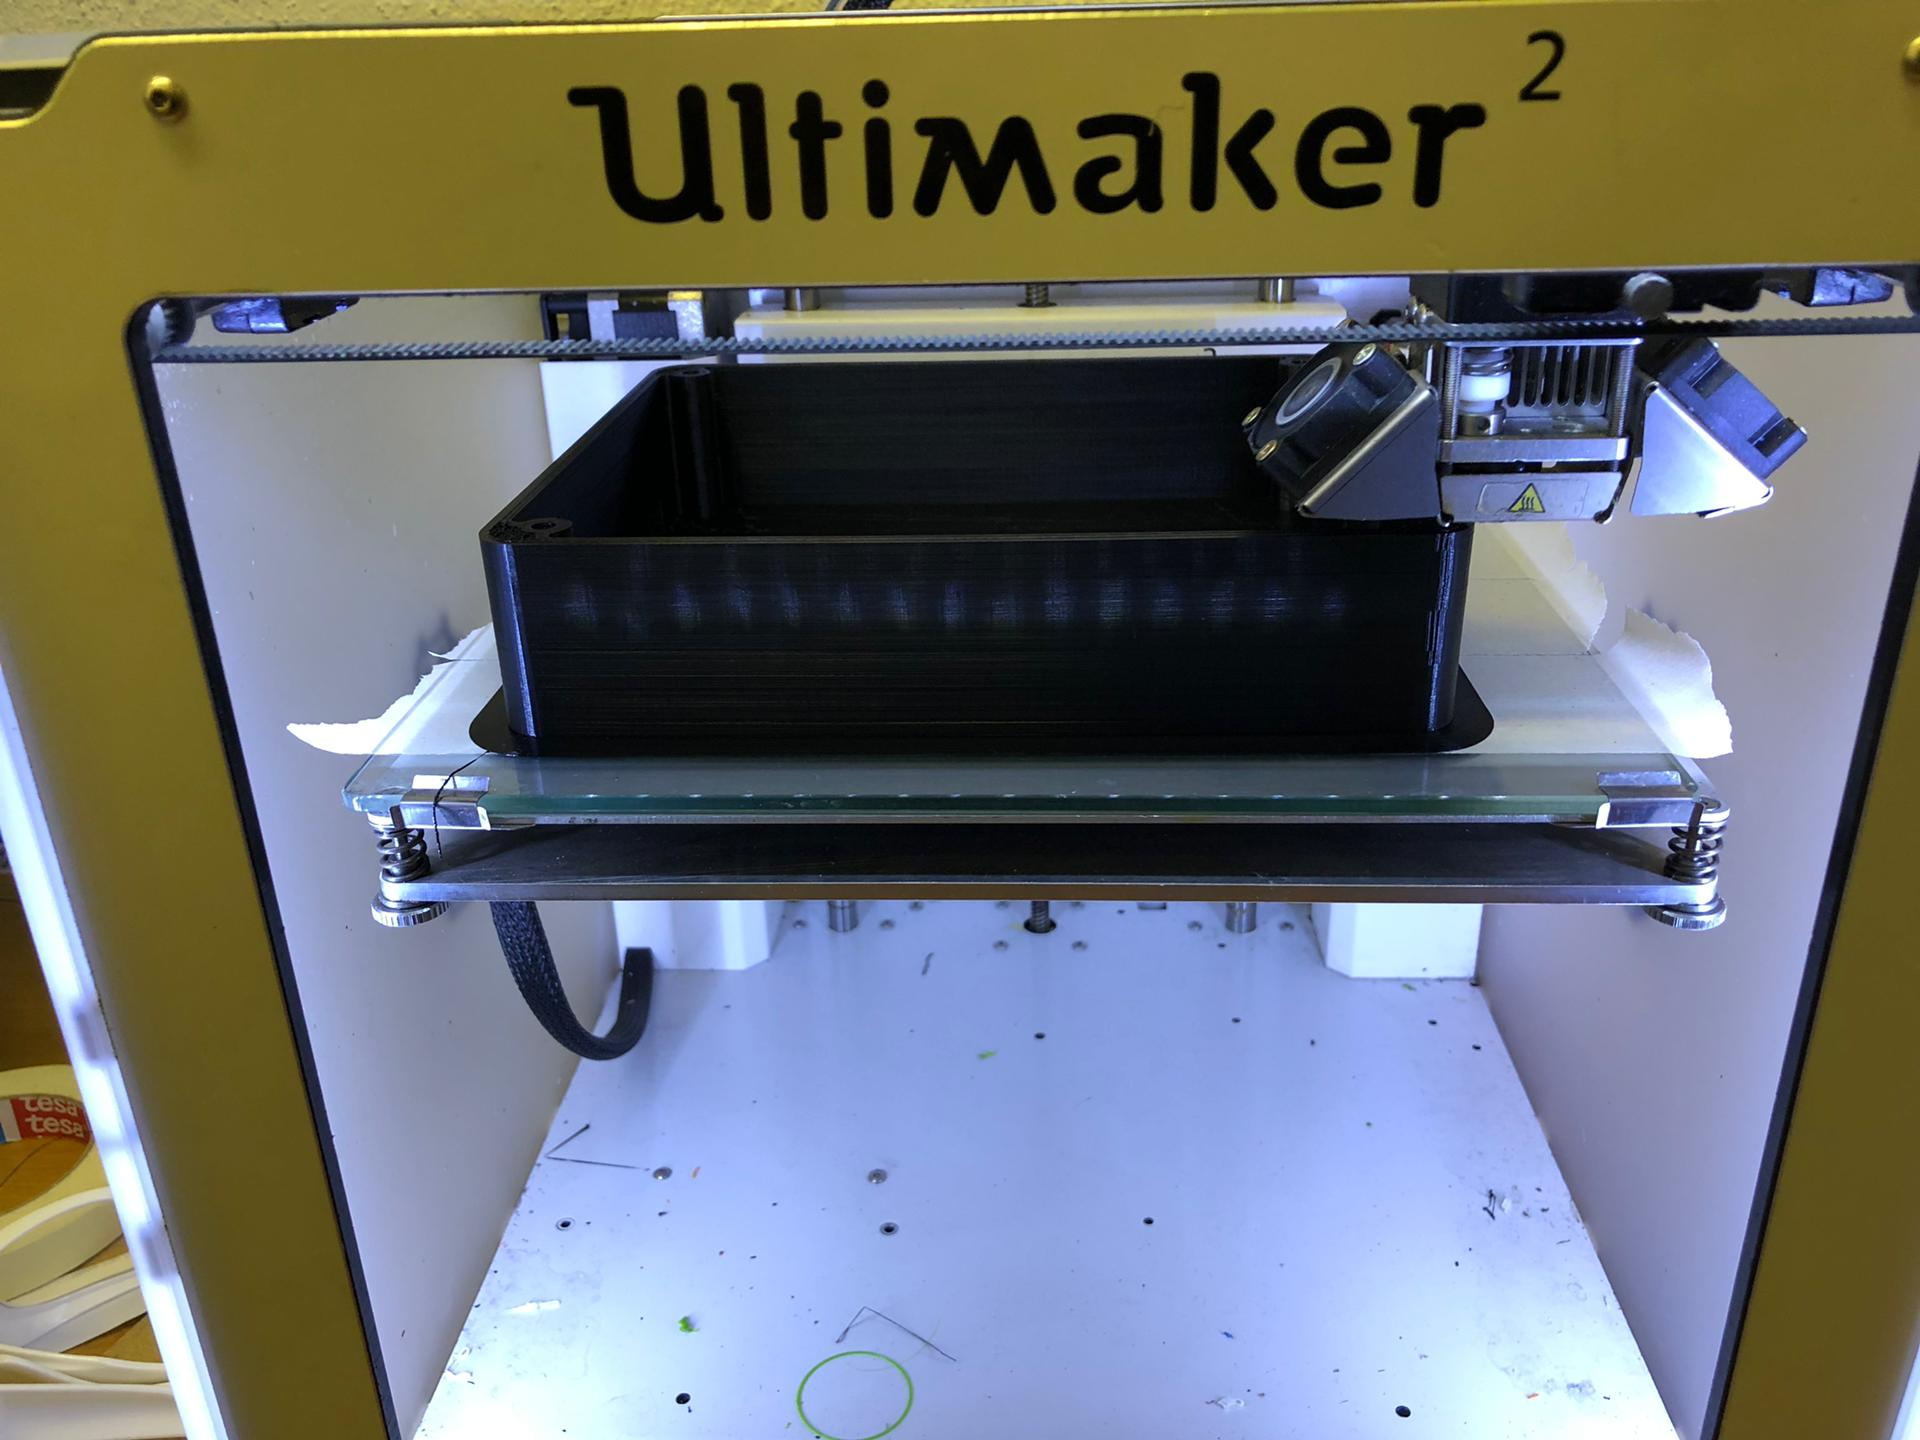
\includegraphics[width=1\textwidth]{Ferni (1).jpg}
\end{center}
\column{0.5\textwidth}
\begin{center}
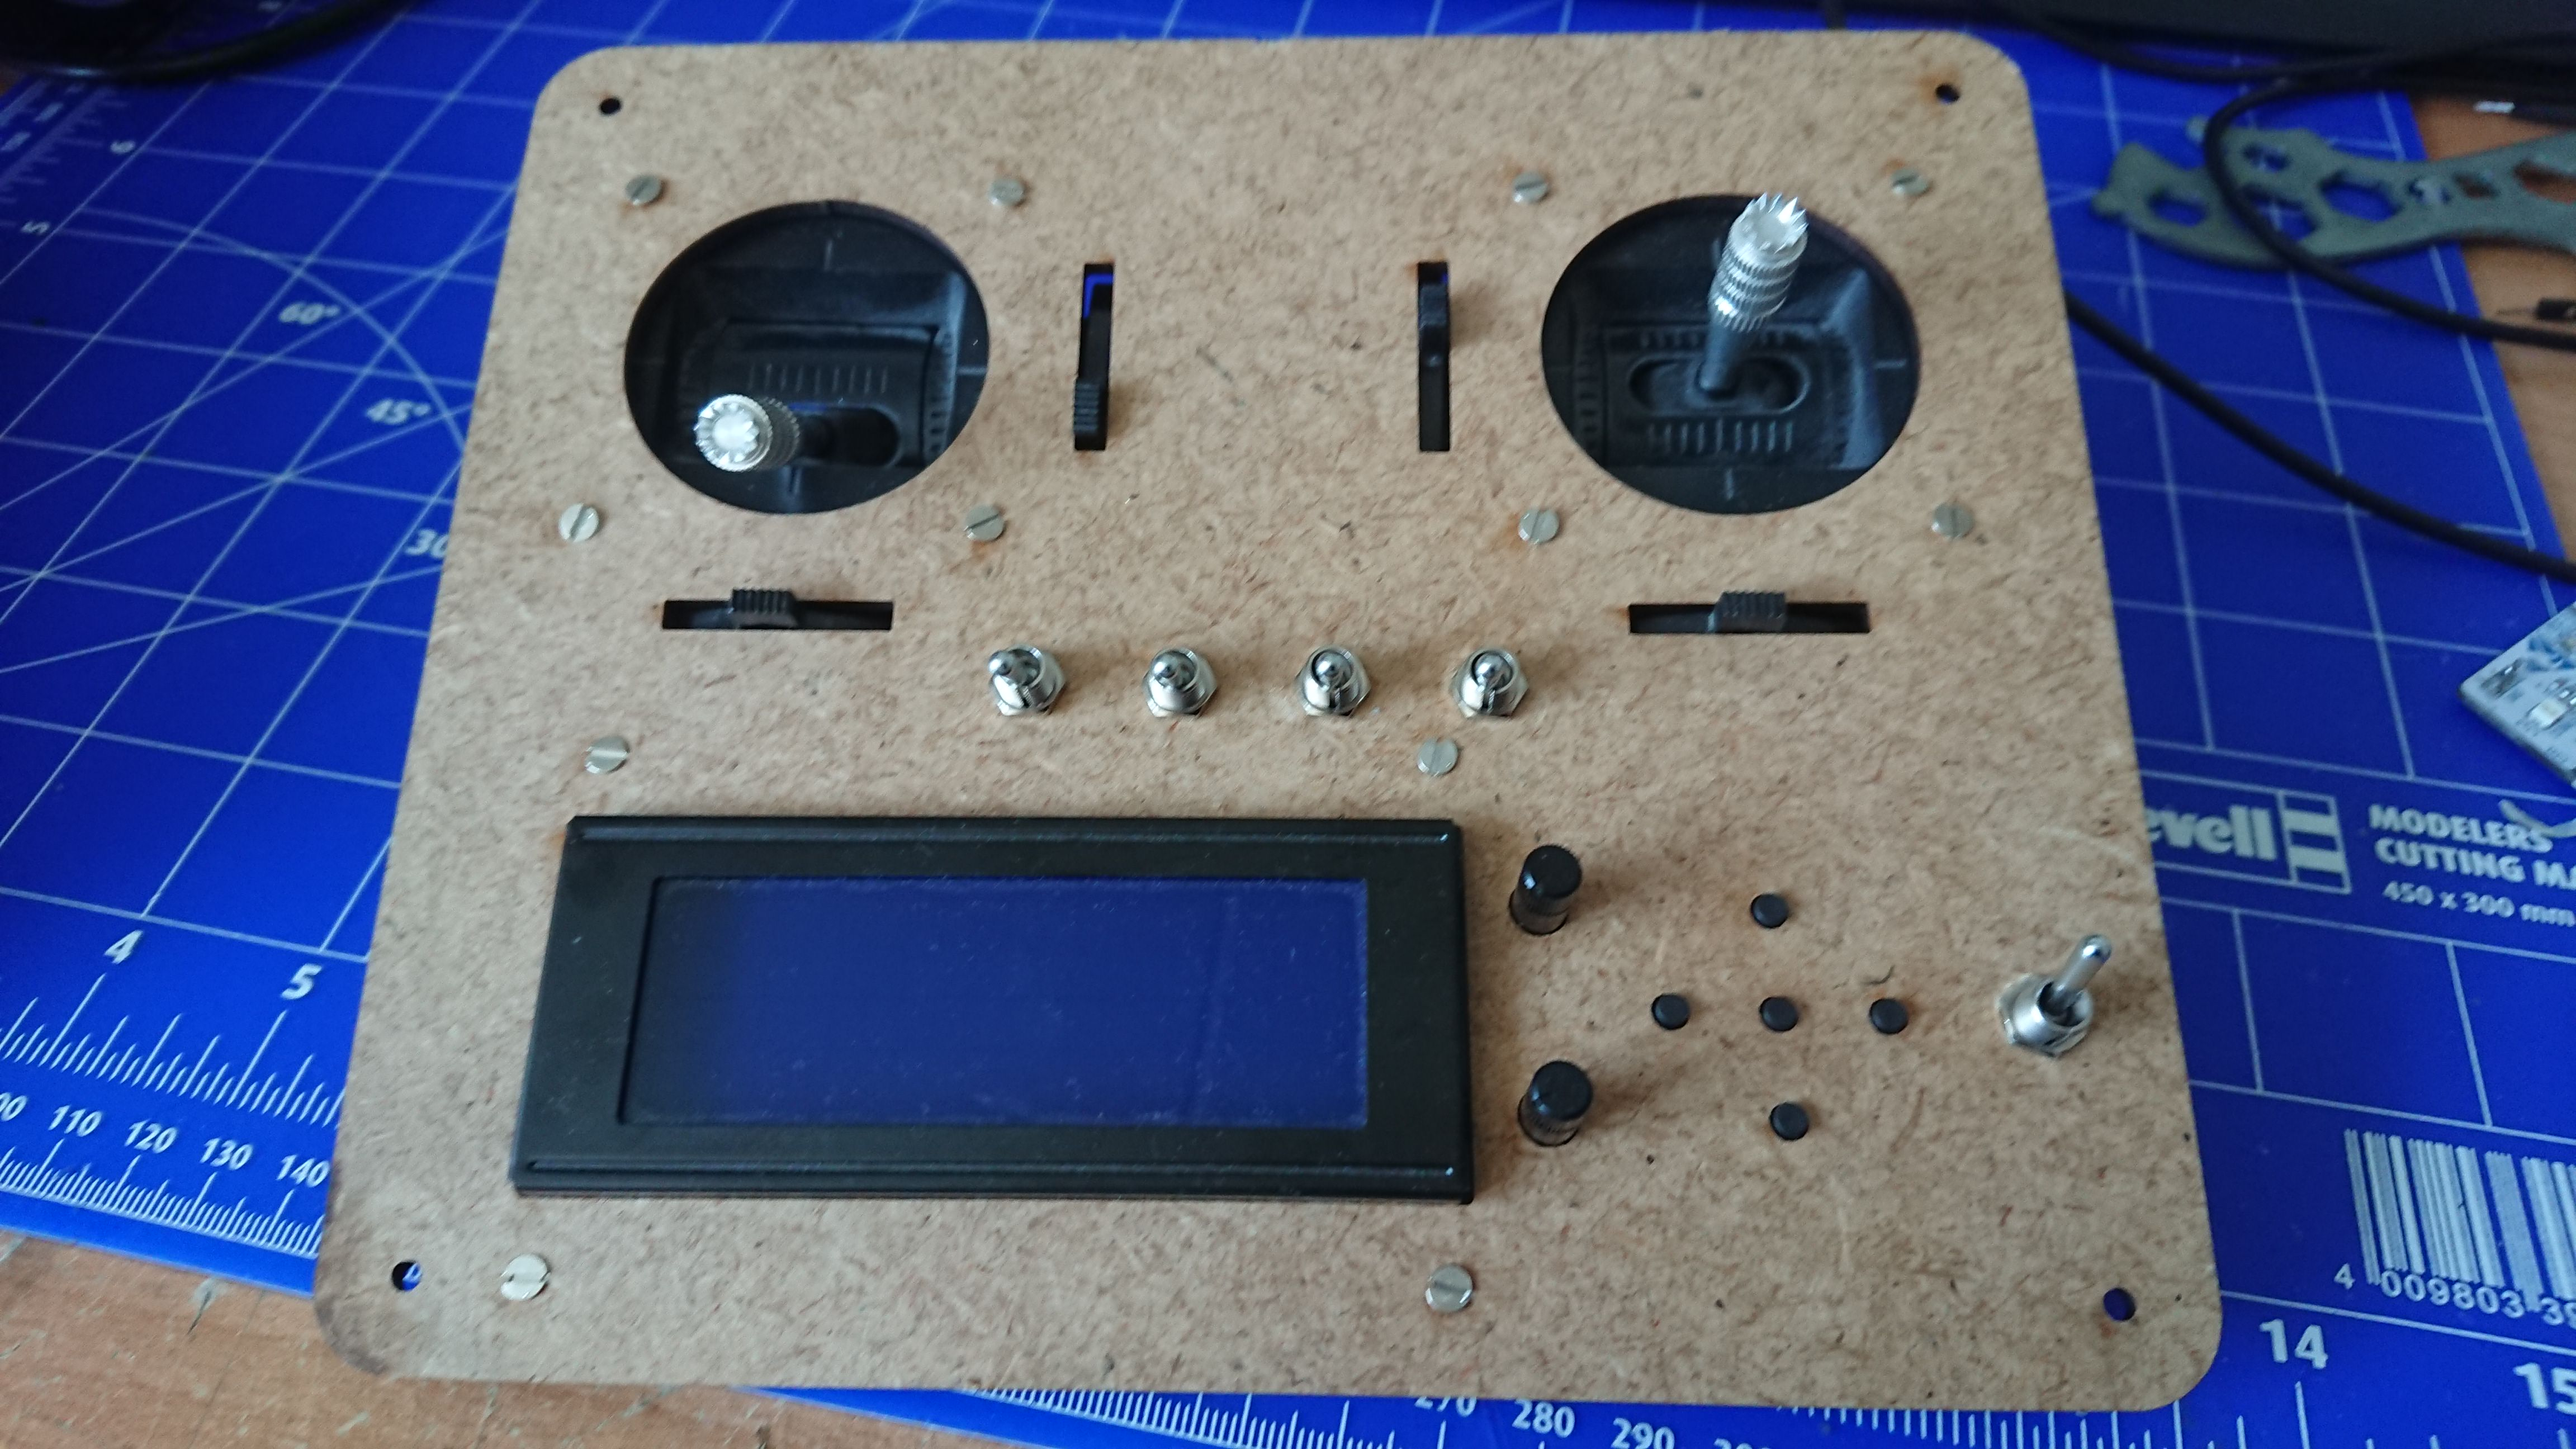
\includegraphics[width=1\textwidth]{Ferni (4).jpeg}
\end{center}
\end{columns}
\end{frame}

\begin{frame}
\frametitle{Bau - Bilder}
\begin{columns}
\column{0.5\textwidth}
\begin{center}
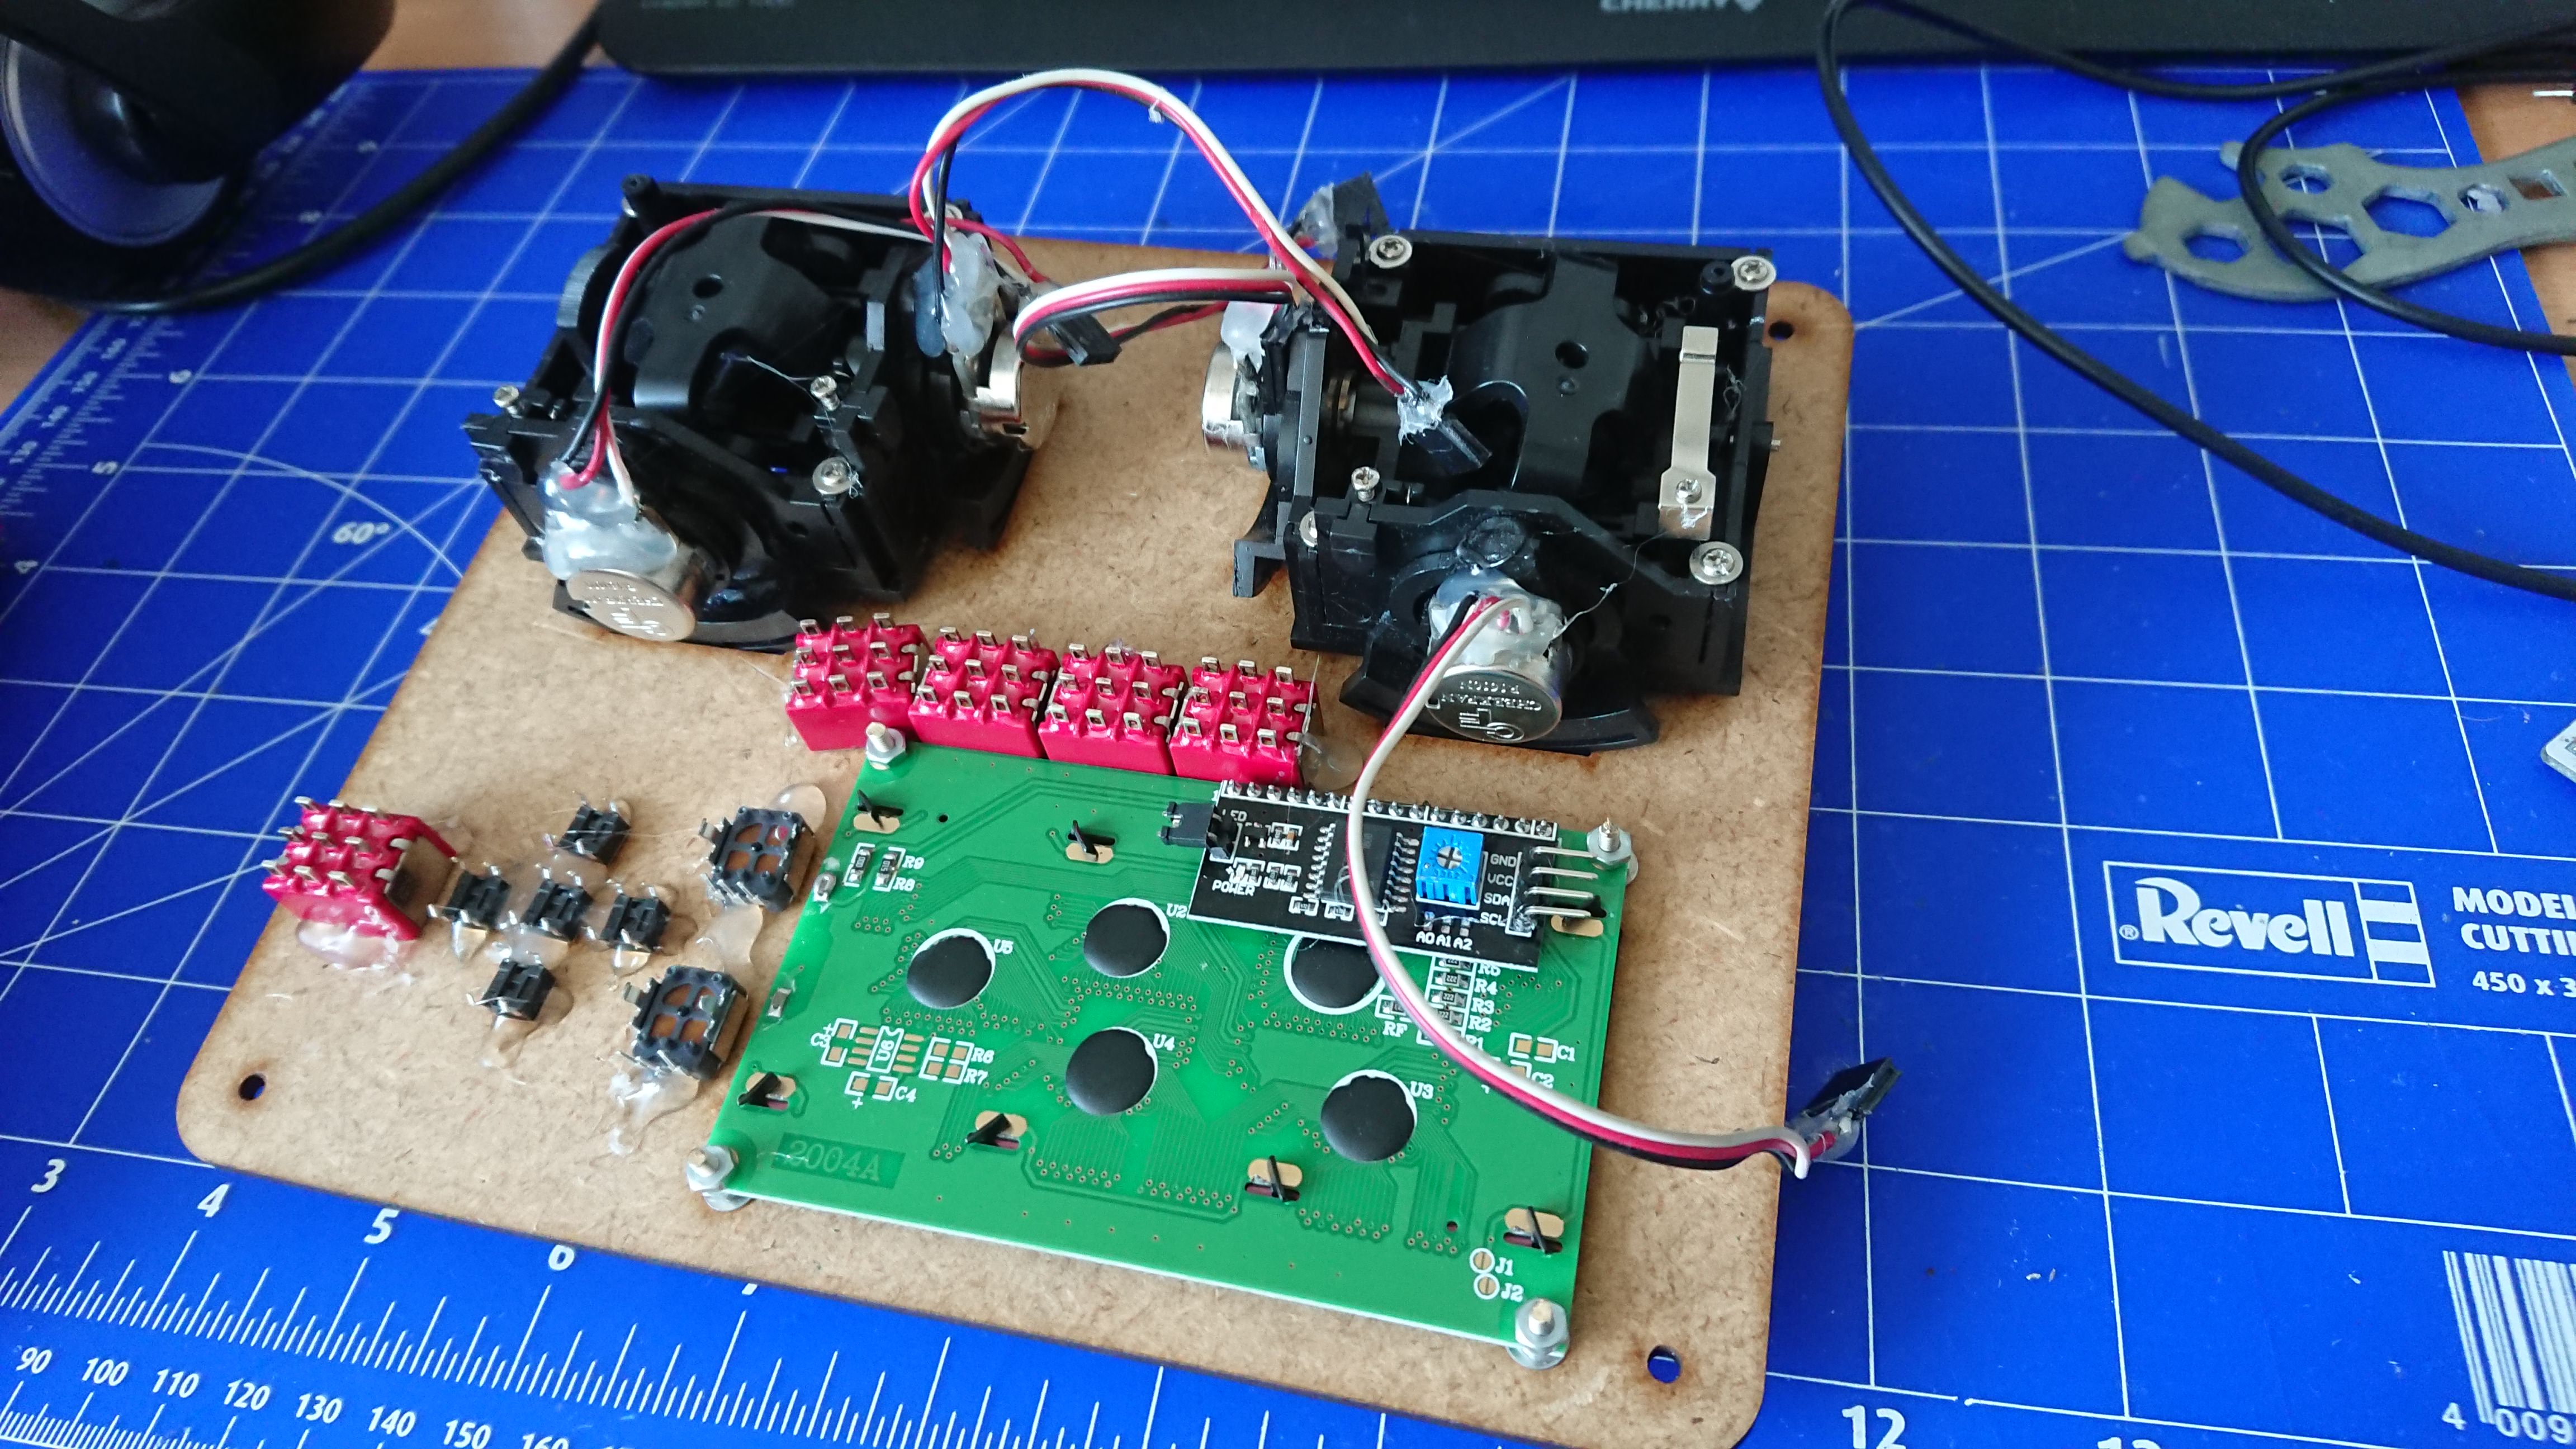
\includegraphics[width=1\textwidth]{Ferni (3).jpeg}
\end{center}
\column{0.5\textwidth}
\begin{center}
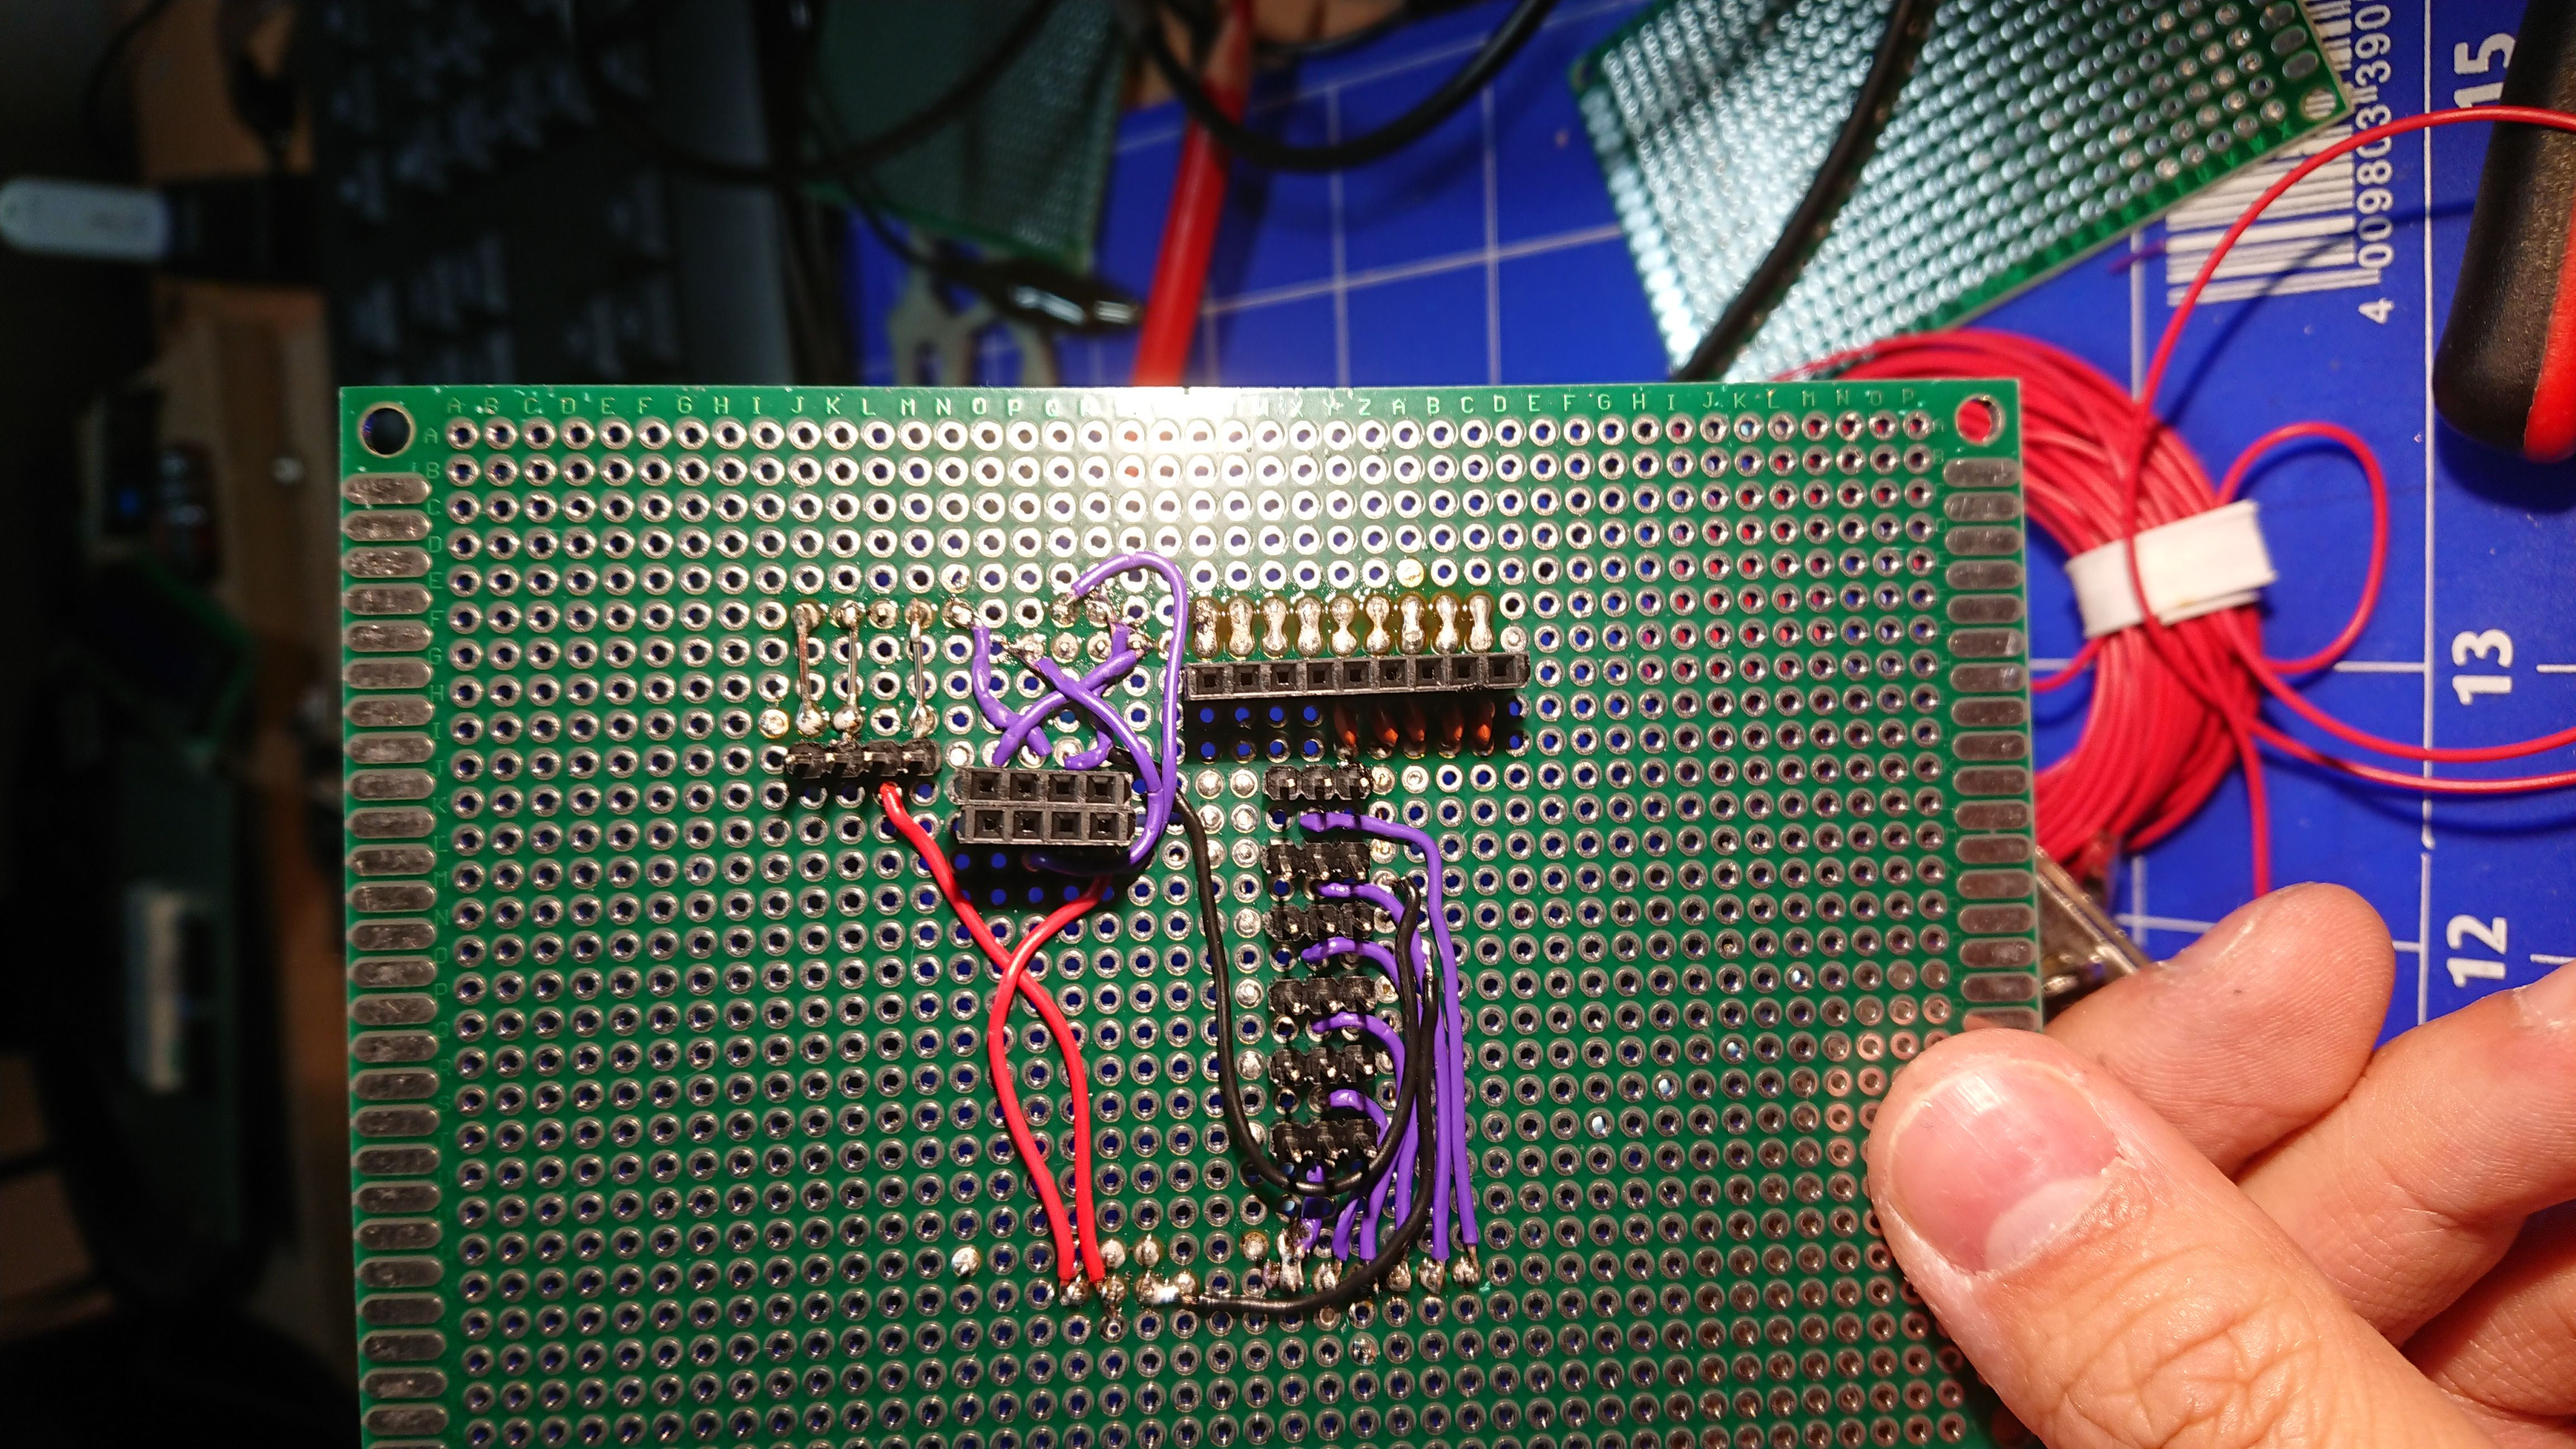
\includegraphics[width=1\textwidth]{Ferni (5).jpeg}
\end{center}
\end{columns}
\end{frame}

\subsection{Programmierung}
 
\begin{frame}
\frametitle{Programmierung}
\begin{columns}
\column{0.5\textwidth}
\begin{itemize}
\item neue Umgebung
\item Zeitkritisch
\item Bugs
\item Debugging
\item langsame math. Funktionen
\end{itemize}
\column{0.5\textwidth}
\begin{center}
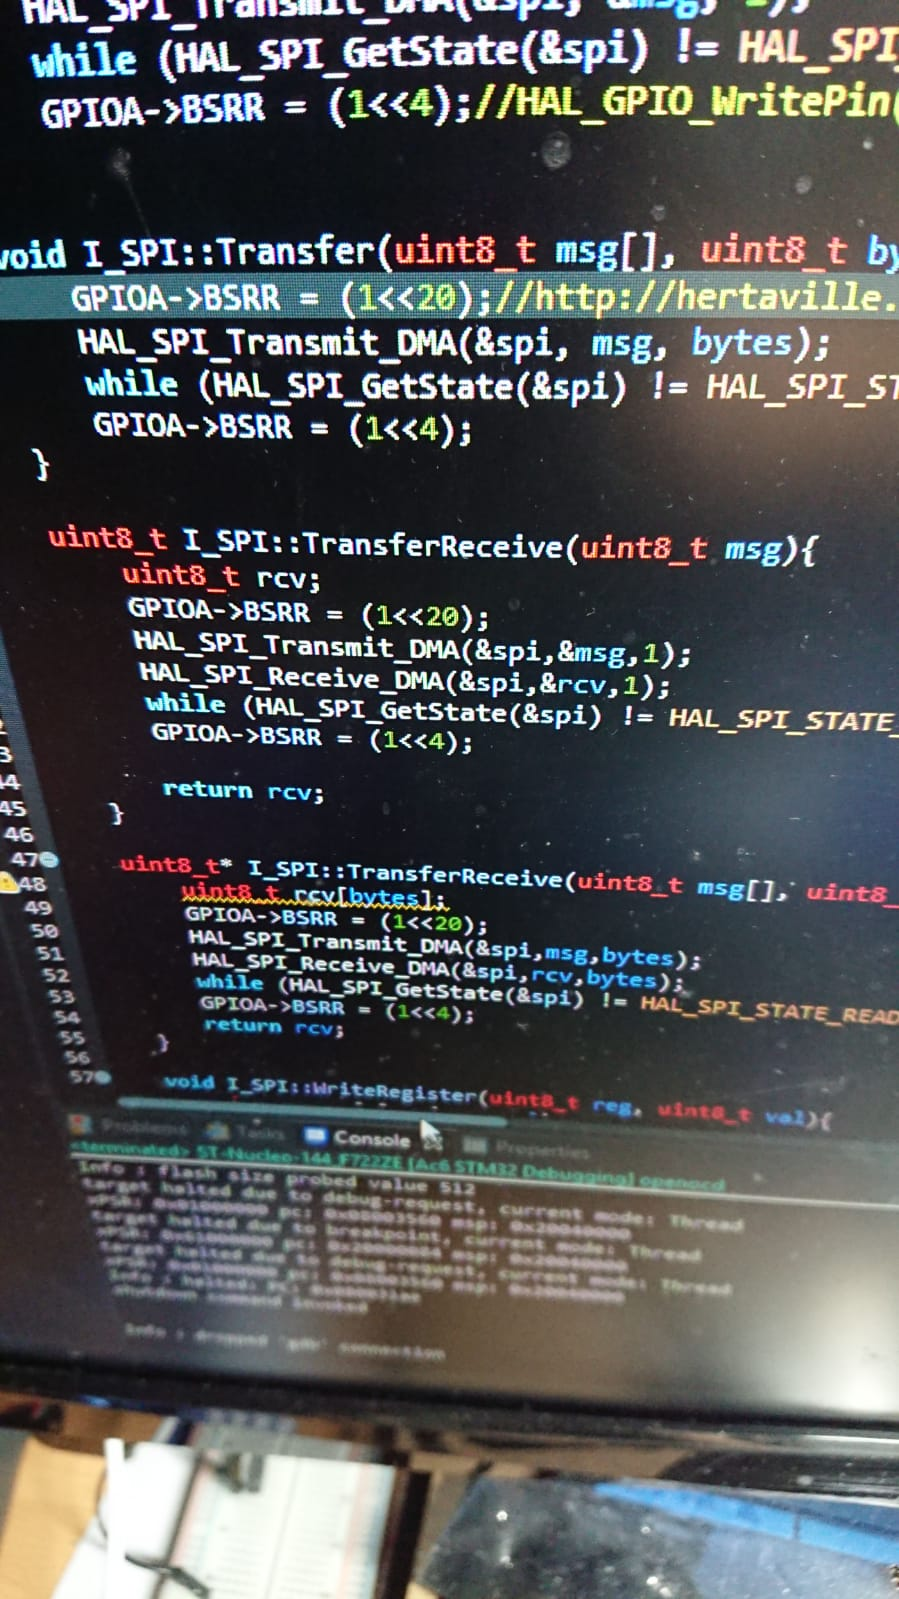
\includegraphics[width=0.7\textwidth]{Prgm1.jpg}
\end{center}
\end{columns}
\end{frame}

\begin{frame}
\begin{alertblock}{Tipp}
Git oder andere Versionsverwaltungsysteme retten Leben!!!
\end{alertblock}
\end{frame}

\section{Filter und PID-Regler}
\subsection{Filter}

\begin{frame}
\frametitle{Filter}
\begin{itemize}
\item beeinflusst Regler
\item verursacht durch Motoren, Assymetrie, etc.
\item verzögert Signal
\item digitalisierter RC-LowPass-Filter
\end{itemize}
\end{frame}

\subsection{PID-Regler}

\begin{frame}
\frametitle{PID-Regler}
\begin{itemize}
\item Reglelkreis
	\begin{itemize}
	\item Messen
	\item Regeln
	\item Stellen
	\end{itemize}
\item 2 Regler (P, I)
\item 1 Glied (D)
\end{itemize}
\end{frame}

\begin{frame}
\frametitle{P-Regler}
\begin{columns}
\column{0.5\textwidth}
\begin{itemize}
\item reagiert schnell
\item schwingt bei zu hohem Wert
\end{itemize}
\column{0.5\textwidth}
\begin{equation*}
y(t)=Kp\cdot e(t)
\end{equation*}
\end{columns}
\end{frame}

\begin{frame}
\frametitle{I-Regler}
\begin{columns}
\column{0.5\textwidth}
\begin{itemize}
\item reagiert langsam
\item schwingt bei zu hohem Wert
\end{itemize}
\column{0.5\textwidth}
\begin{equation*}
y(t)=Ki\int_{0}^{t}e(t)dt
\end{equation*}
\end{columns}
\end{frame}

\begin{frame}
\frametitle{D-Glied}
\begin{columns}
\column{0.5\textwidth}
\begin{itemize}
\item kein richtiger Regler
\item reagiert sehr schnell
\item probleme bei rauschen
\end{itemize}
\column{0.5\textwidth}
\begin{equation*}
y(t)=Kd\cdot \dot{e}(t)
\end{equation*}
\end{columns}
\end{frame}


\begin{frame}
\frametitle{Fragen?}
\end{frame}

\end{document}